% !TeX spellcheck = de_DE
\chapter{Grundlagen}
% !TeX spellcheck = de_DE
\section{Neuronale Netze}
\label{sec:neuroal_networks}
Klassische Algorithmen in der Informatik beschreiben, mit welchen Schritten ein spezielles Problem gelöst werden kann. In vielen Anwendungsfällen, wie zum Beispiel beim Sortieren einer Liste, verwenden Computersysteme diese und lösen das gegebene Problem schneller und effizienter als es Menschen möglich ist. Andere Aufgaben hingegen können von Menschen ohne Aufwand gelöst werden, stellen aber Computersysteme vor große Herausforderungen. Hierzu zählt unter anderem die Klassifizierung von Bildern. Ein Mensch kann beispielsweise Bilder von Hunden und Katzen unabhängig von Blickwinkel und Bildqualität unterscheiden beziehungsweise richtig zuordnen. Trotzdem ist es aufwendig, für solche Probleme klassische Algorithmen zu entwickeln, da die Lösung von vielen subtilen Faktoren abhängt \cite{kriesel2008kleiner}. Häufig werden in diesen Aufgabenfeldern \ac{KNN} eingesetzt, welche von biologischen neuronalen Netzen inspiriert sind und zum Forschungsgebiet des maschinellen Lernens gehören. Auch wenn die \ac{KNN} heute aktuell sind und viel Aufmerksamkeit erhalten, bildet die bereits 1943 veröffentlichte Arbeit von \citeauthor{mcculloch1943logical} die Grundlage für das Forschungsgebiet. In der Arbeit wird ein einfaches neuronales Netz mit Schwellwerten entwickelt, das die Berechnung von logischen und arithmetischen Funktionen ermöglicht \cite{mcculloch1943logical}. In den folgenden Jahrzehnten wurde die Funktionsweise der neuronalen Netze weiterentwickelt und der Einsatz in verschiedenen Aufgabenfeldern ermöglicht. Hierzu zählen neben der Klassifizierung von Bildern \cite{krizhevsky2012imagenet} unter anderem das Erkennen und die Interpretation von Sprache \cite{hinton2012deep}, \cite{andor2016globally} sowie das selbständige Lösen von Computer- und Gesellschaftsspielen \cite{mnih2013playing}, \cite{silver2016mastering}. 
\hl{In diesem Kapitel wird zuerst ...}% TODO Continue
\subsection{Biologische neuronale Netze}
\label{subsec:biological_neuraL_networks}
Das Forschungsgebiet der \ac{KNN} ist von den erfolgreichen biologischen neuronalen Netzen inspiriert, wie zum Beispiel dem menschlichen Gehirn \cite{kriesel2008kleiner}. In diesem Abschnitt werden die Eigenschaften betrachtet, die das Vorbild erfolgreich machen und für die \ac{KNN} übernommen werden sollen. Im Zuge dessen wird ein grober Überblick über die Struktur und Funktionsweise des menschlichen Gehirns gegeben. 
\\\\
Jede Sekunde erfassen die Rezeptoren des menschlichen Körpers unzählige Reize, wie zum Beispiel Licht, Druck, Temperatur und Töne. Die Reize werden anschließend elektrisch oder chemisch kodiert und über Nervenbahnen an das Gehirn geleitet, welches die Aufgabe hat, diese zu filtern, zu verarbeiten und entsprechend zu reagieren. Als Reaktion können zum Beispiel Signale an entsprechende Muskeln oder Drüsen gesendet werden \cite{kinnebrock2018neuronale}. Hierbei zeichnet sich das biologische neuronale Netz durch drei Eigenschaften aus, die klassische Algorithmen entweder nicht besitzen oder nur schwer umsetzen können. Ziel ist es, diese auf die \ac{KNN} zu übertragen \cite{kriesel2008kleiner}.
\begin{enumerate}
	\item \textbf{ Fähigkeit zu Lernen} \\
	Das menschliche Gehirn ist nicht wie ein klassischer Algorithmus für seine Aufgaben programmiert. Stattdessen besitzt es die Fähigkeit, durch Nachahmen oder Ausprobieren zu lernen \cite{kriesel2008kleiner}. Dafür wird das angestrebte Ergebnis mit dem tatsächlich erzielten verglichen und das Verhalten entsprechend angepasst. Dies ermöglicht es Menschen, verschiedene Aufgabengebiete erfolgreich zu lösen und sich ändernden Anforderungen anzupassen.
	
	\item \textbf{Fähigkeit zur Generalisierung}\\
	Auch für unbekannte Situationen findet das Gehirn meist plausible Lösungen, da es die Fähigkeit zur Generalisierung besitzt \cite{kriesel2008kleiner}. Das bedeutet, dass viele Situationen bereits bekannten Problemen zugeordnet werden können, mithilfe derer eine passende Verhaltensstrategie ausgewählt wird. 
	
	\item \textbf{Toleranz gegenüber Fehlern}\\
	Zudem zeichnen sich biologische neuronale Netze durch eine hohe Fehlertoleranz gegenüber verrauschten Daten aus. Beim zuvor genanntem Beispiel der Klassifizierung kann ein Teil des Bildes fehlen oder unscharf sein, trotzdem kann das abgebildete Motiv richtig zugeordnet werden.
\end{enumerate}

\subsubsection{Struktur des menschlichen Gehirns}
Das Forschungsgebiet der Neurowissenschaften befasst sich unter anderem mit dem menschlichen Gehirn, dessen Funktionsweise auch heute noch nicht vollständig erforscht ist. Dennoch ist schon seit 1861 durch die Arbeit von Paul Broca bekannt, dass es im menschlichen Gehirn verschiedene Regionen mit unterschiedlichen Aufgaben gibt \cite{russell2013kunstliche}. Zum Beispiel wird das sogenannte Kleinhirn (Cerebellum) für einen Großteil der motorischen Koordination verwendet, während das Großhirn (Telencephalon) unter anderem visuelle Reize empfängt \cite{kriesel2008kleiner}. Trotz der unterschiedlichen Aufgaben haben alle Bereiche des Gehirns einen gemeinsamen Grundbaustein, die sogenannten Neuronen \cite{russell2013kunstliche}. Im Folgenden wird der Aufbau und die Funktionsweise von diesen oberflächlich in Bezug auf die später vorgestellten künstlichen Neuronen betrachtet. Für einen vollständigen Überblick und eine genaue Beschreibung der Vorgänge ist auf entsprechende Fachliteratur zu verweisen.
\begin{figure}[h]
	\centering
	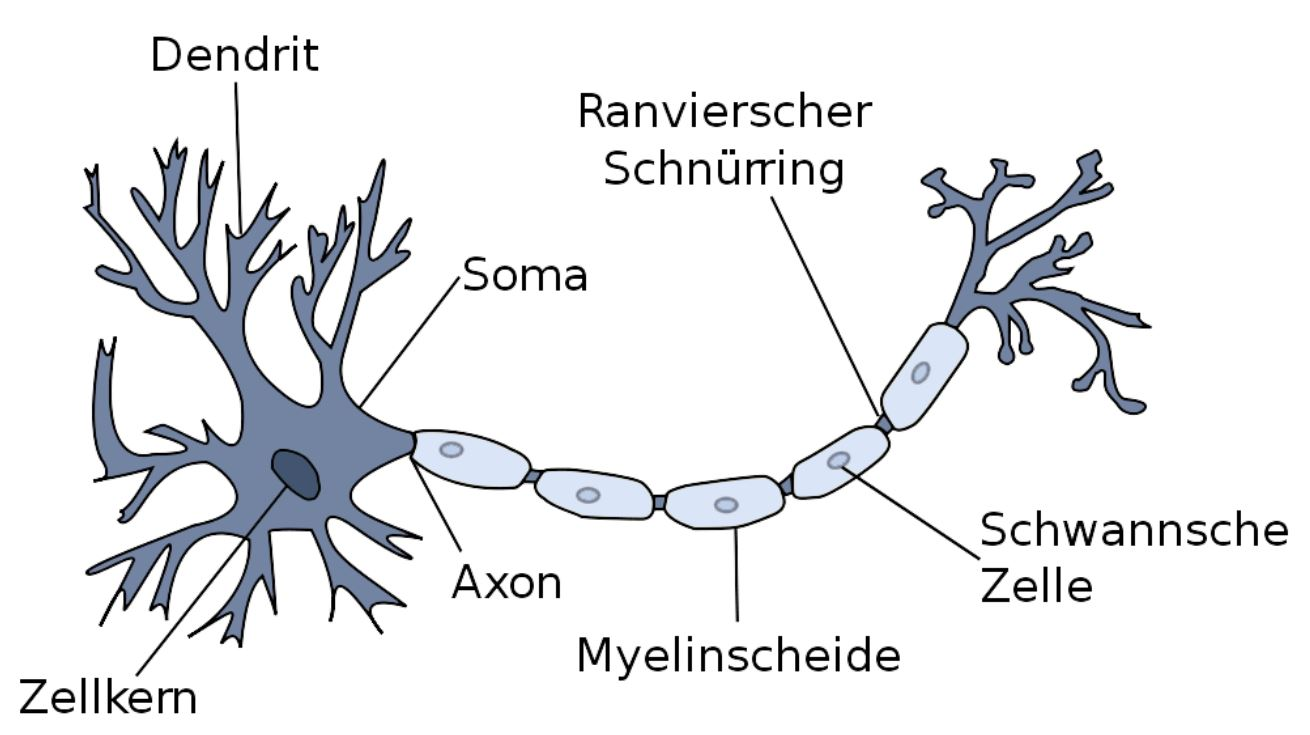
\includegraphics[width=0.75\textwidth]{./img/biologial_neuron.JPG} 
	\caption{Schematische Abbildung einer Nervenzelle \cite{kriesel2008kleiner}.}
	\label{fig:biological_neuron}
\end{figure}
\\ \noindent
Das menschliche Gehirn besitzt ungefähr ${10}^{11}$ einzelne Neuronen, deren schematischer Aufbau in Abbildung \ref{fig:biological_neuron} dargestellt ist. Jedes Neuron besitzt einen Zellkern, der sich im Zellkörper (Soma) befindet. Von dem Zellkörper gehen mehrere Fasern aus, die Dendriten genannt werden \cite{russell2013kunstliche}. An diesen befinden sich Synapsen, welche als Übertragungsstelle fungieren und elektrische oder chemische Signale von Rezeptoren oder anderen Neuronen empfangen \cite{kriesel2008kleiner}. Typischerweise empfängt ein Neuron Signale von 2000 bis 10.000 anderen Nervenzellen \cite{zell2003simulation}.  % TODO 3 mal empfangen
Synapsen, die elektrische Signale erhalten, haben eine starke, direkte, nicht regulierbare Verbindung vom Sender zum Empfänger. Diese sind für hart kodierte Verhaltensmechanismen nützlich, wie zum Beispiel den Fluchtreflex. Die chemische Synapse hingegen ist nicht direkt mit dem Sender verbunden, sondern durch den synaptischen Spalt getrennt. Zur Übertragung eines elektrischen Signals wird dieses auf der präsynaptischen Seite in ein chemisches Signal kodiert, indem Neurotransmitter freigesetzt werden. Diese können über den synaptischen Spalt übertragen und anschließend auf der postsynaptischen Seite wieder in ein elektrisches Signal kodiert werden. Ein großer Vorteil dieser Übertragungsart ist die Regulierbarkeit \cite{kriesel2008kleiner}. Verschiedene Neurotransmitter können unterschiedliche Effekte auf das Neuron haben, beispielsweise anregend (exzitatorisch) oder hemmend (inhibitorisch) wirken \cite{kirschbaum2008biopsychologie}. Zusätzlich kann die Menge der freigesetzten Neurotransmitter die Stärke des Signals beeinflussen \cite{kriesel2008kleiner}. Langfristig gesehen können auch neue Verbindungen bzw. Synapsen entstehen oder alte aufgelöst werden. Es wird angenommen, dass dies die Grundlage des Lernens im menschlichen Gehirn ist \cite{russell2013kunstliche}.
\\\\
Sowohl die anregenden als auch hemmenden Signale werden über die Dendriten an den Axonhügel weitergeleitet, welcher sich zwischen dem Soma und dem Axon befindet. Dort werden die Signale akkumuliert. Beim Überschreiten eines gewissen Schwellwerts wird ein elektrischer Impuls erzeugt, den das Axon weiterleitet \cite{kirschbaum2008biopsychologie}. Das Axon ist typischerweise einen Zentimeter, in Ausnahmen sogar bis zu einem Meter lang und wird von der Myelinscheide umgeben, die unter anderem Schutz vor mechanischer Überbeanspruchung bietet \cite{russell2013kunstliche}. Zusammen mit den Ranvierschen Schnürringen ermöglicht sie zudem eine schnellere Weiterleitung des Aktionspotenzials \cite{kirschbaum2008biopsychologie}. Das Axon endet mit dem sogenannten Endknopf, auch Axonterminal genannt. Dieses ist mit den Synapsen von anderen Neuronen verbunden und setzt beim Eintreffen eines Signals die Neurotransmitter frei, wodurch das Signal übertragen wird \cite{kirschbaum2008biopsychologie}. Typischerweise gibt ein einzelnes Neuron sein Signal an 1000 bis 10.000 andere Neuronen weiter, in Extremfällen sogar an bis zu 150.000 andere Neuronen \cite{zell2003simulation}, die alle parallel arbeiten. So entsteht ein großes und leistungsfähiges neuronales Netz. 

\subsection{Künstliche neuronale Netze}
\ac{KNN} sind ein mathematisches Modell, das im Vergleich zum biologischen Vorbild stark vereinfacht und idealisiert ist. Trotzdem können unterschiedliche mathematische Funktionen abgebildet werden. In diesem Kapitel werden die grundsätzliche Funktionsweise sowie die einzelnen Komponenten der \ac{KNN} vorgestellt.
\begin{figure}[h]
	\centering
	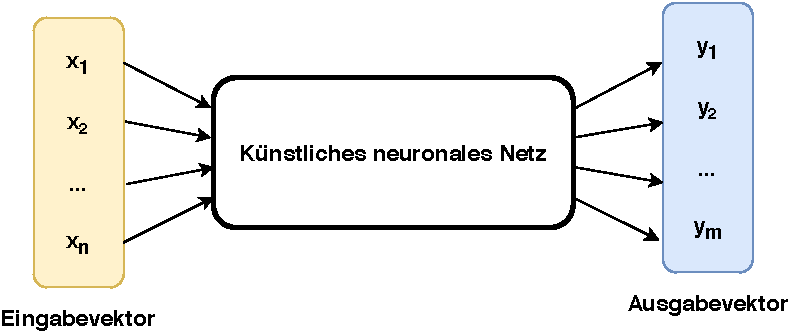
\includegraphics[width=0.6\textwidth]{./img/neural_network_basics/NeuralNetworkBlackbox.pdf} 
	\caption{KNN als Blackbox mit einem Eingabe- und Ausgabevektor}
	\label{fig:neural_network_blackbox}
\end{figure}
\\ \noindent
Betrachtet man ein \ac{KNN} als Blackbox (Abbildung \ref{fig:neural_network_blackbox}), gibt es eine gewisse Anzahl an Eingabewerten, die in einem Eingabevektor kodiert sind und eine Anzahl an Ausgaben, die in einem Ausgabevektor kodiert sind \cite{scherer2013neuronale}. Die Eingaben werden im Fall der \ac{KNN} nicht durch Rezeptoren erfasst, sondern sind durch ein Optimierungsproblem gegeben. Der Ausgabevektor soll das gewünschte Ergebnis enthalten. Je nach Optimierungsproblem kann die Interpretation von diesem variieren. Betrachtet man die Struktur der \ac{KNN}, sind einige Ähnlichkeiten zum biologischen Vorbild erkennbar. Diese werden im Folgenden genauer betrachtet \cite{zell2003simulation}:
\begin{enumerate}
	\item \textbf{Neuronen}\\
	Ähnlich zu den biologischen neuronalen Netzen, besteht auch das \ac{KNN} aus vielen Neuronen \cite{zell2003simulation}. Dies sind einfache Recheneinheiten, die primitive Funktionen bestimmen können \cite{scherer2013neuronale} und deren genaue Funktionsweise in Kapitel \ref{subsec:neuron} erläutert wird. Vorweggenommen sei, dass ein Neuron mehrere Eingabewerte besitzt, welche gewichtet sind und akkumuliert werden. Hierbei entsteht ein skalarer Ausgabewert, der den Aktivierungsgrad des Neurons repräsentiert und von anderen Neuronen als Eingabe verwendet werden kann \cite{kriesel2008kleiner}. 
	 
	\item \textbf{Gerichtete gewichtete Verbindungen}\\
	Wie in der Betrachtung der Neuronen angedeutet, sind diese über gerichtete Verbindungen miteinander vernetzt. Der Aktivierungszustand eines Neurons wird entsprechend der Verbindungen an die Zielneuronen weitergegeben, welche diesen Wert als Eingabe verarbeiten. Wie bei den biologischen neuronalen Netzen auch, können Eingaben unterschiedlich stark anregend oder hemmend wirken. Dies wird bei den \ac{KNN} über Gewichte in den Verbindungen realisiert \cite{zell2003simulation}.
	
	\item \textbf{Struktur und Gewichte}\\
	Der Ausgabevektor eines \ac{KNN} ist abhängig von der Struktur des Netzes und der Gewichte in den einzelnen Verbindungen.
	Für das erfolgreiche Lösen eines Optimierungsproblems muss ein \ac{KNN} die richtige Kombination aus Neuronen, Netzstruktur und gewichteten Verbindungen besitzen. Diese müssen durch Lernverfahren bestimmt werden, auf die in Kapitel \ref{subsec:optimization_strategies} näher eingegangen wird.
\end{enumerate}
Trotz der vorgestellten Ähnlichkeiten sind einige Unterschiede zwischen den biologischen neuronalen Netzen und den \ac{KNN} zu verdeutlichen, für die als Beispiel der Größenunterschied zu nennen ist. Das menschliche Gehirn mit seinen ${10}^{11}$ Neuronen besitzt pro Neuron ungefähr $10^4$ Verbindungen, wogegen die meisten \ac{KNN} nur ${10}^{2}$ bis ${10}^{4}$ Neuronen mit insgesamt ${10}^{5}$ Verbindungen besitzen. Auch werden keine chemischen Effekte, die auf benachbarte Neuronen wirken, sowie zeitliche und räumliche Lokalitätsprinzipien beachtet \cite{zell2003simulation}. Aus diesen Gründen sind die \ac{KNN} keine Nachbildung der biologischen neuronalen Netze, sondern verwenden diese ausschließlich als Inspiration. 

\subsection{Das Neuron}
\label{subsec:neuron}
In diesem Kapitel wird die Funktionsweise der einzelnen Neuronen betrachtet. Hierfür werden drei Phasen, die Propagierungsfunktion, die Aktivierungsfunktion sowie die Ausgabefunktion vorgestellt, in denen der Ausgabewert eines einzelnen Neurons berechnet wird. Betrachtet man ein \ac{KNN}, führen typischerweise mehrere Verbindungen zu einem Neuron $j$, welche von den Neuronen $i_1, i_2, ..., i_n$ ausgehen \cite{kriesel2008kleiner}. Dies ist schematisch in Abbildung \ref{fig:neuron_overview} dargestellt.
\begin{figure}[h]
	\centering
	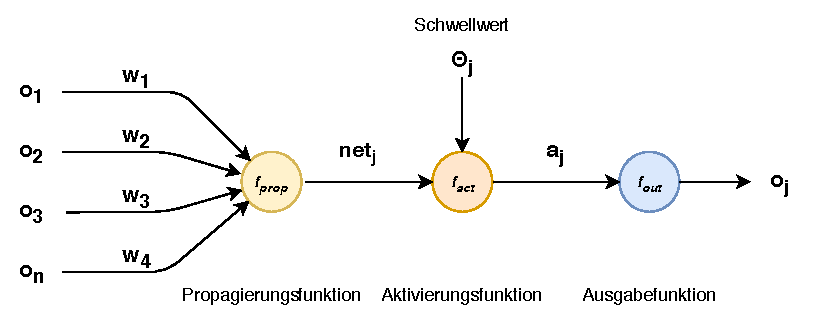
\includegraphics[width=0.9\textwidth]{./img/neural_network_basics/neuron_overview.pdf} 
	\caption{Schematische Darstellung eines einzelnen künstlichen Neurons}
	\label{fig:neuron_overview}
\end{figure}

\subsubsection{Propagierungsfunktion} 
Die Ausgabewerte $o_{i_1}, o_{i_2}, ..., o_{i_n}$ der Neuronen $i_1, i_2, ..., i_n$ werden als Eingabewerte für das Neuron $j$ verwendet. Für jeden Eingabewert existiert ein entsprechendes Gewicht $w_1, w_2, ..., w_n$ \cite{kriesel2008kleiner}. Somit repräsentiert $w_{ij}$ das Gewicht für die Verbindung von Neuron $i$ zu Neuron $j$ \cite{zell2003simulation}. Die Propagierungsfunktion $f_{prop}$ berechnet die Netzeingabe $net_j$, welche in der darauffolgenden Phase weiterverwendet wird \cite{kriesel2008kleiner}. 
$$net_j=f_{prop}(o_1, o_2, ..., o_n, w_1, w_2, ..., w_n)$$
Die meist verwendete Propagierungsfunktion, welche auch in den späteren Beispielen genutzt wird, ist die gewichtete Summe. Hierbei werden entsprechend der Formel die Werte $o_i$ mit dem entsprechenden Gewicht $w_i$ multipliziert und aufsummiert \cite{kriesel2008kleiner}:
$$net_j=\sum_{i}(o_{i} \cdot w_{i, j})$$

\subsubsection{Aktivierungsfunktion}
\label{subsubsec:activatoin_function}
Der Aktivierungszustand $a_j(t)$ gibt den Grad der Aktivierung von Neuron $j$ zum Zeitpunkt $t$ an. Ein neuer Aktivierungszustand zum Zeitpunkt $t+1$ wird mit der Aktivierungsfunktion $f_{act}$ berechnet. Diese berücksichtigt nicht nur die Netzeingabe $net_j(t)$, sondern auch den vorherigen Aktivierungszustand $a_j(t)$ und den Schwellwert $\Theta$ der Aktivierungsfunktion \cite{zell2003simulation}. Ein Schwellwert $\Theta_j$, auch \emph{Bias} genannt, ist dem Neuron $j$ zugeordnet und gibt die Stelle an, an welcher die Aktivierungsfunktion die größte Steigung hat \cite{kriesel2008kleiner}. Somit kann die Berechnung der Aktivierung $a_j(t+1)$ durch folgende Formel ausgedrückt werden \cite{zell2003simulation}:
$$a_j(t+1)=f_{act}(a_j(t), net_j, \Theta_j)$$
Bei der Berechnung kommt dem Schwellwert $\Theta$ eine besondere Bedeutung zu. Oftmals verwenden einige oder alle Neuronen eines \ac{KNN} dieselbe Aktivierungsfunktion, die Schwellwerte hingegen unterscheiden sich je nach Neuron. Des Weiteren sei angemerkt, dass die vorherige Aktivierung $a_j(t)$ je nach Netzstruktur oft keine Berücksichtigung bei der Berechnung findet \cite{kriesel2008kleiner}. Zudem wird in der Praxis bei Verwendung der gewichteten Summe als Propagierungsfunktion der Schwellwert eines Neurons oft schon in der ersten Phase miteinbezogen. Hierdurch ändert sich die Berechnung der Netzeingabe zu $net_j=\sum_{i}(o_{i} \cdot w_{i, j}) - \Theta_j$. Bei der Berechnung der Aktivierungsfunktion gilt dann $\Theta_j = 0$.
\\\\
Je nach Anwendungsgebiet können verschiedene Aktivierungsfunktionen mit unterschiedlichen Eigenschaften eingesetzt werden. Vier Beispiele sind im Folgenden vorgestellt, für die angenommen wird, dass $\Theta_j=0$ ist. Das einfachste Beispiel für eine Aktivierungsfunktion ist die sogenannte binäre Schwellwertfunktion, welche nur die Werte $0$ und $1$ zurückgeben kann \cite{kriesel2008kleiner}. Die Formel hierfür ist: 
$$
f_{act}(net_j)=\left\{\begin{array}{ll}
1 & \text { wenn } net_j \geq 0 \\
0 & \text { wenn } net_j < 0
\end{array}\right.
$$
Allerdings ist für diese Funktion der Wert der Ableitung immer $0$, ausgenommen an dem Schwellwert, an welchem sie nicht differenzierbar ist. Diese Eigenschaften machen sie ungeeignet für bestimmte Lernverfahren, wie zum Beispiel den Backpropagation Algorithmus, auf den in Kapitel \ref{subsec:backprop_algo} kurz eingegangen wird \cite{kriesel2008kleiner}. \\\\
Dieses Problem kann durch die Verwendung einer Sigmoidfunktion gelöst werden. Zwei bekannte Beispiele für Sigmoidfunktionen sind die logistische Funktion und der \ac{tanh} \cite{lecun2012efficient}. Die logistische Funktion kann Werte von 0 bis 1 annehmen und wird berechnet durch \cite{kriesel2008kleiner}: 
$$f_{act}(net_j)=\frac{1}{1+e^{-net_j}}$$
Allerdings können neuronale Netze je nach Verfahren schneller optimiert werden, wenn das durchschnittliche Gewicht aller Verbindungen nahe 0 ist. In diesem Fall kann die \ac{tanh} Funktion besser geeignet sein, da sie Werte zwischen -1 und 1 annehmen kann \cite{lecun2012efficient}. Das abschließend vorgestellte Beispiel ist die sogenannte \emph{Rectifier}-Funktion. Diese wird oft in Zusammenhang mit dem Backpropagation Algorithmus erfolgreich eingesetzt \cite{glorot2011deep}. Berechnet wird sie durch:
$$f_{act}(net_j)= max(0, net_j)$$

\subsubsection{Ausgabefunktion}
Die Ausgabefunktion $f_{out}$ berechnet die Ausgabe $o_j$ von Neuron $j$. Als Eingabewert wird die Aktivierung $a_j$ verwendet \cite{zell2003simulation}. Definiert ist die Funktion durch:
$$o_j = f_{out}(a_j)$$
Ähnlich der Aktivierungsfunktion ist die Ausgabefunktion in der Praxis meist global für alle Neuronen definiert. Als eine solche Ausgabefunktion wird häufig die Identitätsfunktion verwendet, für welche $o_j = a_j$ gilt \cite{kriesel2008kleiner}. Diese kommt auch in den später vorgestellten Beispielen zur Anwendung. Ist die Ausgabe $o_j$ berechnet, kann sie als Eingabewert für andere verbundene Neuronen dienen.

\subsection{Netzstrukturen}
\label{subsec:network_structures}
Aus dem vorherigen Kapitel wird deutlich, dass die Gewichte einen großen Einfluss auf den Ausgabewert eines einzelnen Neurons haben. Der Ausgabevektor eines \ac{KNN} wird zusätzlich von der Anzahl an Neuronen sowie deren Verbindungsstruktur beeinflusst. Dieses Kapitel führt verschiedene Varianten ein, die je nach Optimierungsproblem eingesetzt werden können. 
\\\\
Typischerweise besitzt jedes \ac{KNN} Eingabe- und Ausgabeneuronen. Optional kann ein \ac{KNN} beliebig viele verdeckte Neuronen enthalten. Diese werden auch als \emph{Input}-, \emph{Output}- und \emph{Hidden}-Neuronen bezeichnet \cite{zell2003simulation}. Die Anzahl der Eingabe- und Ausgabeneuronen ist abhängig von der Größe des Eingabe- bzw. Ausgabevektors. Für jedes Element in den Vektoren gibt es ein entsprechendes Neuron.
Bei vielen Netzstrukturen werden die Neuronen des \ac{KNN} verschiedenen Schichten zugeordnet. In der ersten Schicht befinden sich die Eingabeneuronen, in der letzten die Ausgabeneuronen. Dazwischen befinden sich $n$ Schichten mit verdecken Neuronen \cite{zell2003simulation}. 
\\\\
Bei der Berechnung eines \ac{KNN} werden zuerst die Werte des Eingabevektors in die entsprechenden \emph{Input}-Neuronen eingesetzt. Anschließend werden alle Neuronen in einer bestimmten Reihenfolge aktiviert bzw. berechnet. Zuletzt bilden die Werte der \emph{Output}-Neuronen den Ausgabevektor. Die \emph{Hidden}-Neuronen, deren Bezeichnung darin begründet ist, dass ihr Ausgabewert nur ein Zwischenergebnis darstellt und vor dem Anwender verborgen bleibt, befinden sich zwischen den \emph{Input}- und \emph{Output}-Neuronen. Trotzdem sind sie ein elementarer Bestandteil der \ac{KNN} und bestimmen maßgeblich deren Leistungsfähigkeit. Beispielsweise kann ein aus \emph{Input}- und \emph{Output}-Neuronen bestehendes \ac{KNN} nur eine lineare Funktion repräsentieren. Ein \ac{KNN} mit einer ausreichend großen verdeckten Schicht kann jede beliebige kontinuierliche Funktion darstellen. Mit zwei Schichten kann ein \ac{KNN} sogar jede unstetige mathematische Funktion mit beliebiger Genauigkeit abbilden \cite{russell2013kunstliche}. Je nach Art des Verbindungsmusters zwischen den Neuronen werden \ac{KNN} einer von zwei Gruppen zugeordnet. Die erste Gruppe enthält Netze ohne Rückkopplung, welche auch \emph{feedforward}-Netze genannt werden. Die zweite Gruppe sind die sogenannten \emph{recurrent}-Netze, zu welchen \ac{KNN} mit Rückkopplungen gehören \cite{zell2003simulation}.

\subsubsection{Netze ohne Rückkopplung}
Die Definition der \emph{feedforward}-Netze sieht vor, dass es keine Verbindung geben darf, die von einem Neuron $j$ ausgeht und wieder zu sich selbst führt. Dabei ist es irrelevant, ob eine direkte oder indirekte Verbindung über Zwischenneuronen besteht. Es entsteht ein azyklischer Graph \cite{zell2003simulation} und das \ac{KNN} kann infolgedessen keinen internen Zustand besitzen. Für die gleiche Eingabe wird immer dasselbe Ergebnis berechnet. Innerhalb dieser Kategorie gibt es zwei Untergruppen, die ebenenweise verbundenen \ac{KNN} und die \ac{KNN}, welche über sogenannte \emph{shortcut} Verbindungen verfügen.
\begin{figure}[h]
	\centering
	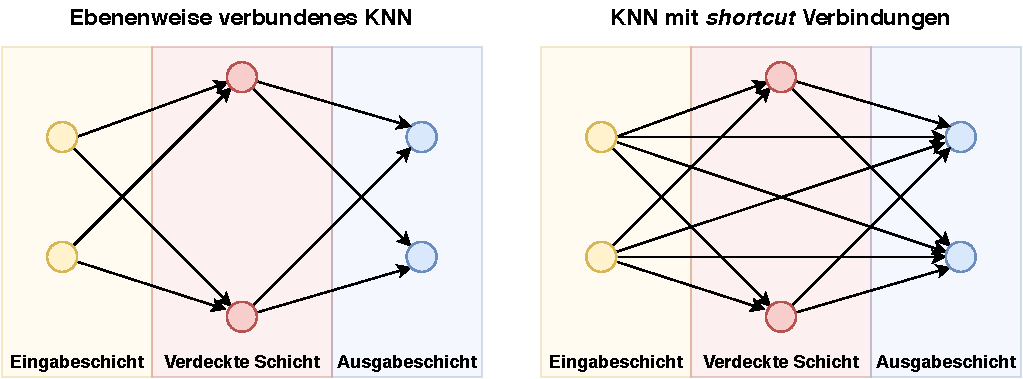
\includegraphics[width=1.0\textwidth]{./img/neural_network_basics/feed_forward_networks.pdf} 
	\caption{Links ein ebenenweise verbundenes \emph{feedforward} KNN, rechts ein KNN mit \emph{shortcut} Verbindungen}
	\label{fig:feed_forward_network_structures}
\end{figure}
Bei den rein ebenenweise verbundenen \ac{KNN} stammen die Eingabewerte eines Neurons immer aus der vorherigen Schicht. Der berechnete Ausgabewert eines Neurons wird nur an die Neuronen der nächsten Schicht weitergeleitet \cite{zell2003simulation}. Ein Beispiel hierfür ist in Abbildung \ref{fig:feed_forward_network_structures} links dargestellt. Im Gegensatz dazu stehen die \ac{KNN} mit \emph{shortcut} Verbindungen. Wie in Abbildung \ref{fig:feed_forward_network_structures} rechts dargestellt, können \emph{shortcut} Verbindungen eine oder mehrere Schichten überspringen. Für gewisse Optimierungsprobleme, unter anderem für das in Kapitel \ref{sec:analysis_valdation_functionality} dargestellte XOR-Problem, können so kleinere \ac{KNN} erzeugt werden \cite{zell2003simulation}. 

\subsubsection{Netze mit Rückkopplung}
Durch rückgekoppelte Verbindungen entstehen Zyklen in der Berechnung, wodurch sich das \ac{KNN} selbst beeinflussen kann. Damit ist unter anderem das Zwischenspeichern von Ergebnissen möglich \cite{russell2013kunstliche}. Somit kann die Berechnung des Ausgabevektors sowohl durch die Eingabewerte als auch durch die vorherigen Ergebnisse beeinflusst werden \cite{lin1998embedded}. Wie die \emph{feedforward}-Netze können auch die Netze mit Rückkopplungen je nach Verbindungsart verschiedenen Untergruppen zugeordnet werden \cite{zell2003simulation}. Diese sind in Abbildung \ref{fig:recurrent_network_structures} dargestellt und im Folgenden beschrieben.
\begin{figure}[h]
	\centering
	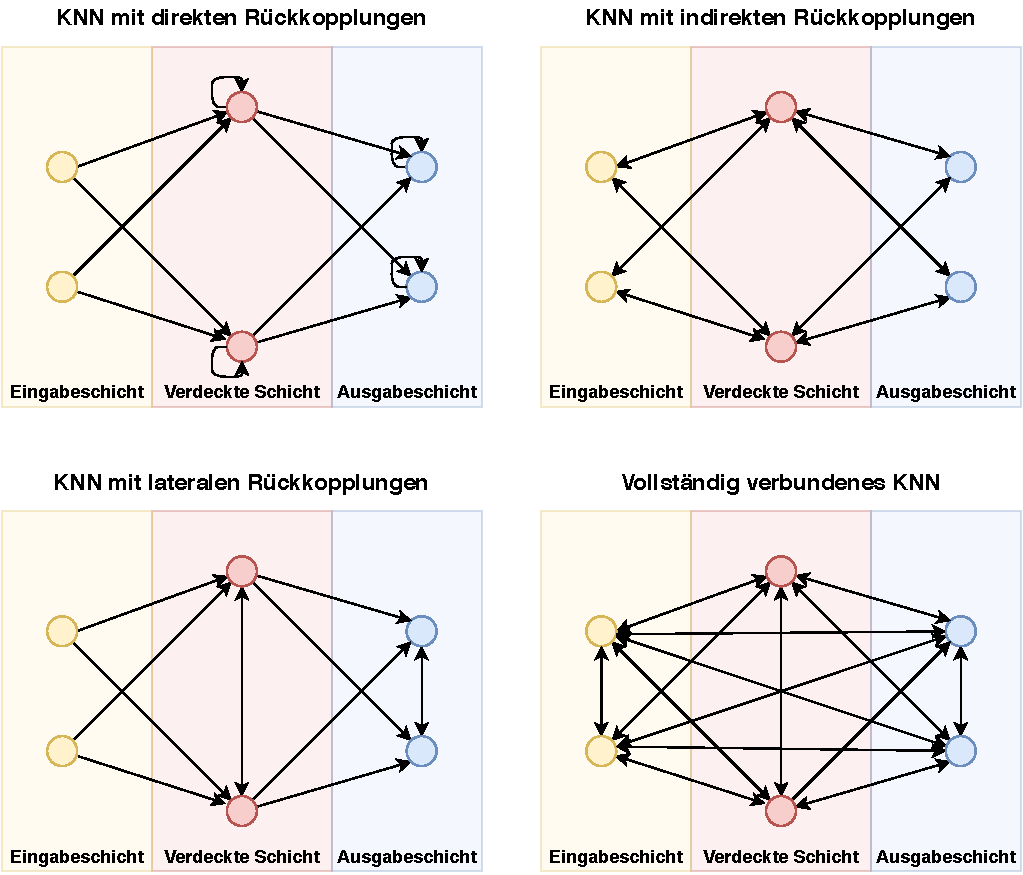
\includegraphics[width=1.0\textwidth]{./img/neural_network_basics/recurrent_networks.pdf} 
	\caption{Schematische Darstellung des Verbindungsmusters von verschiedenen KNN mit Rückkopplungen}
	\label{fig:recurrent_network_structures}
\end{figure}
\begin{enumerate}
	\item Bei \ac{KNN} mit direkten Rückkopplungen können Neuronen Verbindungen zu sich selbst haben und hierdurch ihre eigene Aktivierung verstärken oder abschwächen \cite{zell2003simulation}.
	\item Netze mit einer indirekten Rückkopplung erlauben im Gegensatz zu den \emph{feedforward}-Netzen auch Verbindungen in die vorherige Schicht \cite{zell2003simulation}. Wie bei der direkten Rückkopplung kann sich ein Neuron $j$ selbst beeinflussen, wenn es seinen Ausgabewert an ein Neuron $i$ der nächsten Schicht weiterleitet, welches eine Rückkopplung zu $j$ hat \cite{kriesel2008kleiner}.
	\item \ac{KNN} mit lateralen Rückkopplungen erlauben Verbindungen von Neuronen innerhalb einer Schicht, welche hemmend oder aktivierend wirken können. Oft entsteht dabei ein \emph{Winner-Takes-All}-Schema, da das beste Neuron alle anderen hemmt und sich selbst aktiviert \cite{kriesel2008kleiner}.
	\item Bei den vollständig verbundenen Netzen darf ein Neuron zu jedem anderen eine Verbindung besitzen. Ein Sonderfall sind hier die sogenannten Hopfield-Netze. Bei diesen müssen die Neuronen zu jedem anderen eine Verbindung besitzen mit Ausnahme zu sich selbst \cite{kriesel2008kleiner}.  
\end{enumerate}

\subsection{Optimierungsmöglichkeiten}
\label{subsec:optimization_strategies}
In den vorherigen Kapiteln ist aufgezeigt, dass das erfolgreiche Lösen eines Optimierungsproblems mit einem \ac{KNN} von vielen Faktoren abhängt. In der Praxis ist eine manuelle Bestimmung dieser bei komplexen Aufgaben nicht möglich. Aus diesem Grund muss ein Optimierungsverfahren, welches auch als Lernverfahren bezeichnet wird, angewendet werden. Ziel von diesem ist, einen Teil oder alle Parameter des \ac{KNN} durch einen Algorithmus automatisch zu bestimmen. Typischerweise ist das Lernverfahren unabhängig vom eigentlichen Optimierungsproblem und kann daher in verschiedenen Bereichen ohne großen zusätzlichen Aufwand eingesetzt werden. 
\\\\
Ein Lernverfahren kann theoretisch auf vier verschiedene Arten die Eigenschaften eines \ac{KNN} optimieren \cite{zell2003simulation}. Diese sind im Folgenden kurz zusammenfasst.
\begin{enumerate}
	\item \textbf{Modifizieren der Verbindungsgewichte}:\\
	Die Gewichte der einzelnen Verbindungen werden in der Praxis von allen Lernverfahren optimiert \cite{zell2003simulation}. Gründe hierfür sind, dass ein \ac{KNN} mehrere Millionen Verbindungen besitzen kann, welche unmöglich manuell optimiert werden können, und dass die Gewichte entscheidend für die erfolgreiche Optimierung sind.

	\item\textbf{Modifizieren der Schwellwerte}:\\
	Die Schwellwerte der Neuronen werden wie die Gewichte von den meisten Lernverfahren optimiert. In der Praxis ist der hierbei verwendete Vorgang oft identisch mit der Gewichtsoptimierung. Dies ist möglich, wenn, wie in einigen Implementierungen umgesetzt, die Schwellwerte durch Gewichte repräsentiert werden. Hierzu wird einem \ac{KNN} ein sogenanntes \emph{Bias}-Neuron hinzugefügt, welches immer den Wert 1 hat. Von diesem gehen Verbindungen zu allen Neuronen aus. Der Schwellwert $\Theta_j$ von einem Neuron $j$ wird durch das Gewicht $w_{\Theta j}$ repräsentiert. Dieses ist der eingehenden Verbindung vom \emph{Bias}-Neuron zugeordnet, sodass gilt $1\cdot w_{\Theta j} = \Theta_j$. Dadurch muss bei der Berechnung eines Neurons der Schwellwert nicht mehr explizit miteinbezogen werden, sondern wird im Rahmen der Propagierungsfunktion indirekt mit den anderen gewichteten Eingaben verarbeitet. Bezüglich der Optimierung wird die Verbindung zum \emph{Bias}-Neuron wie andere gewichtete Verbindungen behandelt \cite{zell2003simulation}.

	\item \textbf{Hinzufügen und Entfernen von Verbindungen oder Neuronen}:\\
	Das Hinzufügen beziehungsweise Entfernen von Verbindungen und Neuronen ist im Vergleich zu den bereits vorgestellten Möglichkeiten aufwändig und in der Umsetzung schwieriger. Daher ist es in vielen bekannten Algorithmen nicht implementiert. Bei diesen muss die Struktur mithilfe von Expertenwissen oder Erfahrung festgelegt werden \cite{stanley2017oreilly}, andernfalls ist eine geeignete Struktur experimentell zu ermitteln. Da dieses Vorgehen häufig nicht effizient ist, gibt es dennoch einige Algorithmen, die das Hinzufügen und Entfernen von Strukturen bei der Optimierung nutzen. Diese gehören oft zu der Klasse der neuroevolutionären Algorithmen, auf welche in Kapitel \ref{subsec:neuroevolution} eingegangen wird \cite{kriesel2008kleiner}.
	
	\item \textbf{Ändern der Propagierungs-, Aktivierungs- und Ausgabefunktion}:\\
	Die Optimierung der verwendeten Propagierungs-, Aktivierungs- und Ausgabefunktion ist theoretisch möglich, die Umsetzung ist in der Praxis allerdings nicht sehr verbreitet \cite{zell2003simulation}. Auch in dieser Arbeit werden diese Funktionen nicht durch einen Algorithmus angepasst und daher nicht weiter betrachtet. 
\end{enumerate}

\subsection{Arten von Optimierungsverfahren}
\label{subsec:learning_in_neural_networks}
In Kapitel \ref{subsec:optimization_strategies} sind Optimierungsmöglichkeiten aufgelistet, welche von einem Lernverfahren in der sogenannten Trainingsphase des \ac{KNN} angepasst werden können. Ziel ist, dass am Ende dieser Phase der Ausgabevektor des \ac{KNN} dem gewünschten Ergebnis entspricht. Voraussetzung hierfür ist, dass das gewünschte Ergebnis erkennbar ist \cite{zell2003simulation}. Bei den Lernverfahren wird grundsätzlich zwischen dem überwachten, unüberwachten und bestärkenden Lernen differenziert, welche unterschiedliche Arten des Lernens für verschiedene Aufgabenstellungen repräsentieren. Im Folgenden wird ein Überblick über diese gegeben. Für eine genaue Beschreibung und die dazugehörigen Algorithmen wird auf entsprechende Fachliteratur verwiesen.

\subsubsection{Überwachtes Lernen}
\label{subsubsec:supervised_learning}
Das überwachte Lernen, auch \emph{supervised learning} genannt, wird häufig mit dem Backpropagation Algorithmus und seinen Derivaten umgesetzt und beruht auf bekannten Beispieldaten. Diese müssen in großer Anzahl schon vor dem Lernvorgang vorhanden sein und den Eingabevektor sowie den gewünschten Ausgabevektor des \ac{KNN} enthalten \cite{zell2003simulation}. In der sogenannten Trainingsphase, analysiert das Lernverfahren die vorhanden Beispieldaten mit dem Ziel Muster zu extrahieren. Am Ende der Trainingsphase soll das \ac{KNN} nicht nur die korrekte Lösung für die bekannten Beispiele angeben können, sondern auch für ähnliche, unbekannte Eingabedaten. Damit ist die Eigenschaft der Generalisierung erfüllt. \cite{zell2003simulation}. Um den Erfolg des Verfahrens zu überprüfen, werden die Beispieldaten in Trainings- und Testdaten unterteilt. Die Trainingsphase wird nur mit den Trainingsdaten durchgeführt, sodass die Testdaten dem \ac{KNN} unbekannt sind. Ist diese Phase abgeschlossen, weil beispielsweise das \ac{KNN} eine gute Genauigkeit erreicht hat, werden die Testdaten zur Validierung eingesetzt. Hierbei wird überprüft, ob das \ac{KNN} auch für unbekannte Eingabevektoren die richtigen Ergebnisse berechnet \cite{kriesel2008kleiner}. Diese Art des Lernens ist im Vergleich zu den anderen Varianten sehr schnell \cite{zell2003simulation}, aber das Anwenden ist nicht in jeder Situation möglich. Liegen keine Beispiele vor, kann das \ac{KNN} nicht trainiert werden. Sind die Beispieldaten fehlerhaft oder verrauscht, kann das Training langsam, nicht zufriedenstellend oder unmöglich sein.

\subsubsection{Unüberwachtes Lernen}
\label{subsubsec:unsupervised_learning}
Beim unüberwachten Lernen, auch \emph{unsupervised learning} genannt, stehen ebenfalls Beispieldaten zur Verfügung, allerdings enthalten diese nur den Eingabevektor und keine dazugehörigen Ausgabevektoren. Ziel solcher Lernverfahren ist, Muster in den Eingabedaten automatisch zu erkennen und diese verschiedenen Gruppen zuzuordnen, sodass sich ähnelnde Eingabewerte derselben Gruppe zugewiesen werden \cite{zell2003simulation}. Solche Verfahren können einige Vorteile gegenüber dem überwachten Lernen bieten \cite{mahmad2005IEEE}. Zum Beispiel müssen vor dem Training keine Beispieldaten mit Ausgabevektoren vorliegen, welche teilweise sehr teuer und aufwendig zu erstellen sind. Des Weiteren kann je nach Algorithmus die Anzahl an vorhandenen Gruppen automatisch zugewiesen werden. So können auch unterschwellige Muster, die nicht von einem Menschen erkannt werden würden, die Zuweisung beeinflussen \cite{mahmad2005IEEE}.
 
\subsubsection{Bestärkendes Lernen}
\label{subsubsec:reinforcment_learning}
Die letzte Klasse ist das bestärkende Lernen, auch \emph{reinforcment learning} genannt. Typischerweise wird diese Art des Lernens in dynamischen Umgebungen eingesetzt, in welcher ein sogenannter Agent mit einer Umgebung interagiert. Ein häufig genannter Begriff in diesem Kontext ist der \ac{MDP}, welcher in Abbildung \ref{fig:mdp_problem} dargestellt ist und anhand dessen im Folgenden das bestärkende Lernen beschrieben ist \cite{sutton2018reinforcement}. 
\begin{figure}[h]
	\centering
	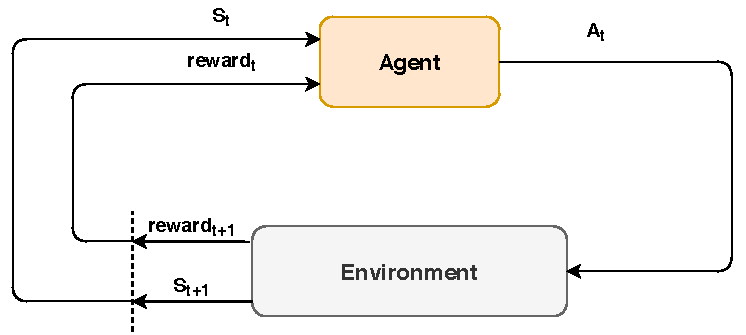
\includegraphics[width=0.7\textwidth]{./img/neural_network_basics/mdp.pdf} 
	\caption{Interaktion des Agenten mit der Umgebung im MDP}
	\label{fig:mdp_problem}
\end{figure}
\\ \noindent
Zwei wichtige Grundkomponenten des \acp{MDP} sind der Agent und die Umgebung. Der aktuelle Zustand der Umgebung zu einem Zeitpunkt $t$ wird durch die Variable $S_t$ repräsentiert. Ist die Umgebung zum Beispiel ein Computerspiel, kann $S_t$ unter anderem die aktuelle Position sowie Zielkoordinaten enthalten. Der Zustand $S_t$ steht dem Agenten zur Verfügung, der daraufhin eine Aktion $A_t$ ausführt. Als Basis für die Entscheidung kann ein \ac{KNN} dienen, welches als Eingabevektor den aktuellen Zustand verwendet und einen Ausgabevektor mit der gewählten Aktion erzeugt. Die verfügbaren Aktionen sind je nach System unterschiedlich. So können zum Beispiel bei der Steuerung von Robotern sowohl direkte Steuersignale für die Motoren ausgegeben werden als auch \emph{high-level} Entscheidungen wie die Bewegungsrichtung. Nach Ausführung der Aktion wird der Zustand der Umgebung entsprechend angepasst und ein neuer Zustand $S_{t+1}$ entsteht \cite{sutton2018reinforcement}, für den der Agent eine neue Aktion auswählen kann. Zusätzlich wird ein Belohnung, auch als $reward$ bezeichnet, vergeben. Dies ist ein numerischer Wert, der angibt, wie richtig oder falsch die gewählte Aktion war \cite{zell2003simulation}. Eine richtige Aktion zeichnet sich dadurch aus, dass sie den Agenten näher an sein gewünschtes Ziel bringt. Im zuvor genannten Beispiel des Computerspiels ist der \emph{reward} größer, wenn der Agent die Distanz zum Ziel verringert und kleiner bzw. negativ, wenn der Agent sich wieder entfernt. Ziel eines Optimierungsalgorithmus ist, die Summe der erhaltenen Belohnungen zu maximieren. Hierdurch ergeben sich komplexe Anforderungen an das Lernverfahren. Bei der Entscheidung, welche Aktion $A_t$ bei einem Zustand $S_t$ den meisten Erfolg verspricht, muss sowohl der direkte als auch zukünftige \emph{reward} berücksichtigt werden \cite{sutton2018reinforcement}. Dies ist notwendig, da ein Agent viele Aktionen in derselben sich ändernden Umgebung ausführt und eine Entscheidung Auswirkungen auf die Zukunft hat. Somit kann es bei vielen Optimierungsproblemen  lohnenswert sein, zur Schaffung einer besseren Ausgangslage zuerst eine schlechte Belohnung in Kauf zu nehmen, sodass im weiteren Verlauf größere Belohnungen erreicht werden können. Eine weitere Herausforderung für solche Algorithmen ist, dass ein Gleichgewicht zwischen dem Nutzen von Erfahrung und Ausprobieren gefunden werden muss. Möglichst hohe Belohnungen kann ein Agent nur erhalten, wenn er bekannte Entscheidungen trifft, die in der Vergangenheit erfolgreich waren. Allerdings müssen auch neue unbekannte Aktionen ausgewählt werden, da diese unter Umständen besser sein können. Für ein gutes Lernverfahren ist es notwendig, eine Kombination aus beidem zu ermöglichen \cite{sutton2018reinforcement}. Bei vielen Optimierungsproblemen wird das bestärkende Lernen erfolgreich eingesetzt. Ein Nachteil jedoch ist die lange Laufzeit im Vergleich zu anderen Verfahren, wie zum Beispiel dem überwachtem Lernen. Grund hierfür ist, dass eine niedrige Belohnung keine Aussage darüber trifft wie das \ac{KNN} optimiert werden soll um bessere Ergebnisse zu erzielen. Anpassungen können sich sowohl positiv als auch negativ auf den Agenten auswirken \cite{zell2003simulation}. 


\subsection{Backpropagation Algorithmus}
\label{subsec:backprop_algo}
???

%Während der Optimierung erhält das \ac{KNN} Beispieldaten, für welche der Ausgabevektor berechnet wird. Für das berechnete %Ergebnis wird ein Feedback gegeben, welches auch als \emph{reward} bezeichnet wird. Dieses gibt an, ob der Ausgabewert korrekt %ist beziehungsweise wie richtig oder falsch. Das Lernverfahren muss mit diesen Angaben das \ac{KNN} optimieren, kann aber nicht %wissen wie die Gewichte und je nach Algorithmus die Struktur verändert werden müssen. Dies ist auch der Grund, warum diese Art %des Lernens im Vergleich zum überwachtem Lernen sehr langsam ist, da die Gewichte nicht gezielt angepasst werden können %\cite{zell2003simulation}.\\
%Das Einsatz

% Agent Scenario, Agent must explore/take known actions = trade off, Reward funktion ist anpassbar, muss nicht so sein. 
% file:///D:/Dropbox/Studium%20Master/Semester%203/Masterthesis%20Quellen/Neuroevolution%20strateies%20for%20episodic%20reinforcment%20learning.pdf
% "C:\Users\Simon Hauck\Downloads\Neuroevolution strateies for episodic reinforcment learning.pdf"


% Sources to check if somewhere available: 
% 1. Simulation neuronaler Netze: https://link.springer.com/book/10.1007/978-3-322-83200-9
% 2. Theorie der neuronalen Netze: Eine systematische Einführung: https://www.springer.com/de/book/9783540563532 check if newer version is available
% 3. Neuronale Netze: Grundlagen und Anwendung: https://www.springer.com/de/book/9783528054656
% https://www.springer.com/de/book/9783528054656
% DONE - Ein kleiner Überblick über neuronale Netze: http://www.dkriesel.com/_media/science/neuronalenetze-de-zeta2-2col-dkrieselcom.pdf
% DONE - Verteilte, evolutionäre Optimierung von Schwärmen http://www.dkriesel.com/_media/science/diplomarbeit-de-1column-11pt.pdf 
% 6. Künstliche Intelligenz und Optimierung https://link.springer.com/chapter/10.1007/978-3-658-02292-1_2
% 7. Neuronale Netze: Eine Einführung in die Neuroinformatik https://www.springer.com/de/book/9783519022473
% DONE - Künstliche Intelligenz Wissensverarbeitung - Neuronale Netze
% DONE - Mathematik für Wirtschaftsinformatiker
% DONE - Multivariate Analysemethoden
% DONE - Künstliche Intelligenz - Wissensverarbeitung - Neuronale netze
\section{Evolutionäre Algorithmen}
\subsection{Genome und Phenom}
\subsection{Phasen des Algos}
\subsection{Kodierung}
\subsection{Competing Convention Problem}
% !TeX spellcheck = de_DE
\section{NeuroEvolution of Augmenting Topologies}
\label{sec:neat}
Der in dieser Arbeit verwendete Algorithmus heißt \ac{NEAT}, welcher im Jahr 2002 von \citeauthor{stanley2002evolving} vorgestellt wurde. Bei der Veröffentlichung hat \ac{NEAT} für die meisten Optimierungsprobleme im Vergleich zu anderen Verfahren schneller Lösungen gefunden, obwohl es neben den Gewichten des \ac{KNN} auch die Struktur optimiert \cite{stanley2002evolving}. Somit gehört der Algorithmus zur Gruppe der \ac{TWEANN} Algorithmen. Heute gilt \ac{NEAT} immer noch als einer der bekanntesten Vertretern der neuroevolutionären Algorithmen und dient als Basis für viele Erweiterungen wie zum Beispiel HyperNEAT, cgNEAT, ... \\
% TODO Add NEAT Sources
Für die guten Ergebnisse sind drei Eigenschaften besonders relevant \cite{stanley2002evolving}:
\begin{enumerate}
	\item Erfolgreiche Reproduktion trotz verschiedener Strukturen
	\item Schützen von neuen Innovationen durch verschiedene Spezies
	\item Wachsen einer minimalen Struktur
\end{enumerate}
In diesem Kapitel wird die grundsätzliche Funktionsweise von \ac{NEAT} erläutert, wie sie in der originalen Publikation vorgestellt ist. Wenn nicht anderweitig gekennzeichnet, beziehen sich alle Informationen aus diesem Kapitel auf Quelle \cite{stanley2002evolving}. Für eine bessere Lesbarkeit wird in diesem Kapitel auf weitere Zitierungen verzichtet.
\subsection{Kodierung}
\label{subsec:neat_encoding} % TODO ABBILDUNG
\begin{figure}[!h]
	\centering
	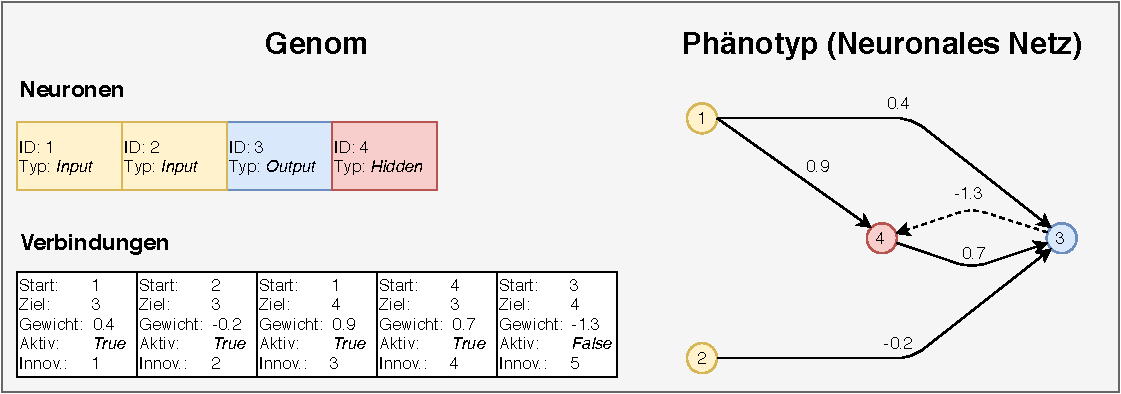
\includegraphics[width=1\textwidth]{./img/neat_genome_encoding.pdf} 
	\caption{Schematische Darstellung von einem Genom mit dazugehörigem Phänotyp}
	\label{fig:neat_encoding}
\end{figure}
\ac{NEAT} verwendet ein direktes Kodierungsverfahren. Ein Genom enthält, wie in Abbildung (TODO ABBILDUNG) beispielhaft dargestellt, je eine Liste für Neuronen und Verbindungen. Ein Neuron wird durch eine ID identifiziert und enthält den Typ (\emph{Input}, \emph{Output}, \emph{Hidden}). Eine Verbindung enthält das Start- und Zielneuron, das dazugehörige Gewicht, ein Aktivierungsbit sowie eine Innovationsnummer. Das Aktivierungsbit gibt an, ob die Verbindung im Phänotyp, in diesem Fall dem neuronalen Netz enthalten, ist. Auf die Funktionsweise und Bedeutung der Innnovationsnummer wird später genauer eingegangen.
\subsection{Mutation}
\label{subsec:neat_mutation}
Ein Genom kann auf verschiedene Arten mutieren, welche entweder die Struktur des \ac{KNN} oder die Gewichte der Verbindungen beeinflussen. Die Mutation der Gewichte ist ähnlich zu anderen neuroevolutionären Algorithmen. Für jedes Gewicht besteht eine Wahrscheinlichkeit zur Mutation. In diesem Fall wird das Gewicht entweder leicht abgeändert oder ein neuer zufälliger Wert gewählt.\\ % TODO ABBILDUNG
\begin{figure}[!h]
	\centering
	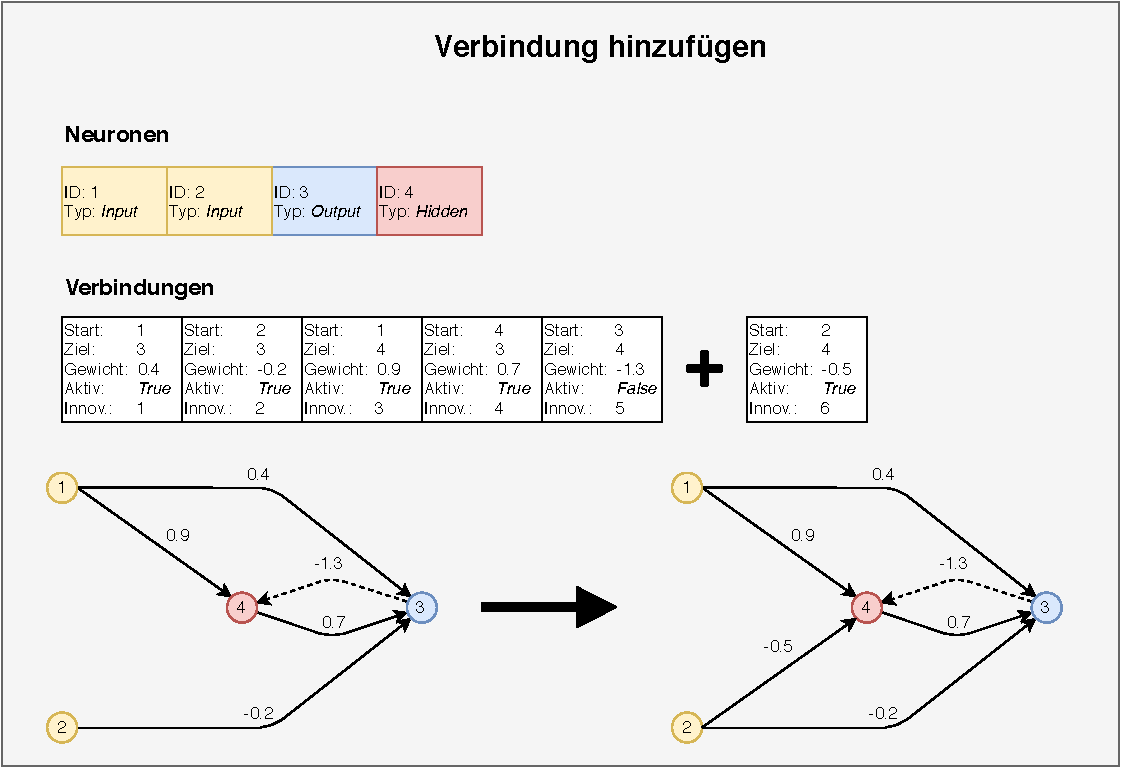
\includegraphics[width=1\textwidth]{./img/neat-AddConnectionMutation.pdf} 
	\caption{Schematische Darstellung von einem Genom mit dazugehörigem Phänotyp}
	\label{fig:neat_add_connectin_mutation}
\end{figure}
Strukturelle Mutationen können in zwei verschiedenen Arten auftreten. Bei der ersten wird eine einzelne neue Verbindung dem Genom hinzugefügt. Bei der Auswahl des Start- und Zielneurons ist zu beachten, dass diese nicht bereits über eine solche Verbindung verfügen. Das Gewicht für die neue Verbindung wird zufällig gewählt und das Aktivierungsbit auf \emph{True} gesetzt. Ein Beispiel für diese Mutation ist in Abbildung (TODO ABBILDUNG) dargestellt. Bei der zweiten Art der strukturellen Mutation wird ein neues Neuron in das \ac{KNN} eingefügt. Hierzu wird zu Beginn eine aktive Verbindung $con_{ij} $ zufällig ausgewählt, welche von Neuron $i$ zu Neuron $j$ führt. Anschließend wird ein neues Neuron $x$ zwischen den Neuronen $i$ und $j$ platziert und zwei weitere Verbindungen werden hinzugefügt. Die erste Verbindung $con_{ix}$ führt vom alten Startneuron $i$ zum neu hinzugefügtem und erhält das Gewicht $1$. Die zweite Verbindung $con_{xj}$ beginnt bei dem neuen Neuron und endet im dem alten Zielneuron $j$ und erhält dasselbe Gewicht wie die Verbindung $con_{ij}$. Zuletzt wird die ausgewählte Verbindung $con_{ij}$ deaktiviert, indem das Aktivierungsbit auf $False$ gesetzt wird. Diese Art der Mutation reduziert den initialen Effekt des neuen Neurons. So kann es direkt vom \ac{KNN} verwendet werden, ohne dass die Verbindungsgewichte stark optimiert werden müssen.
\begin{figure}[!h]
	\centering
	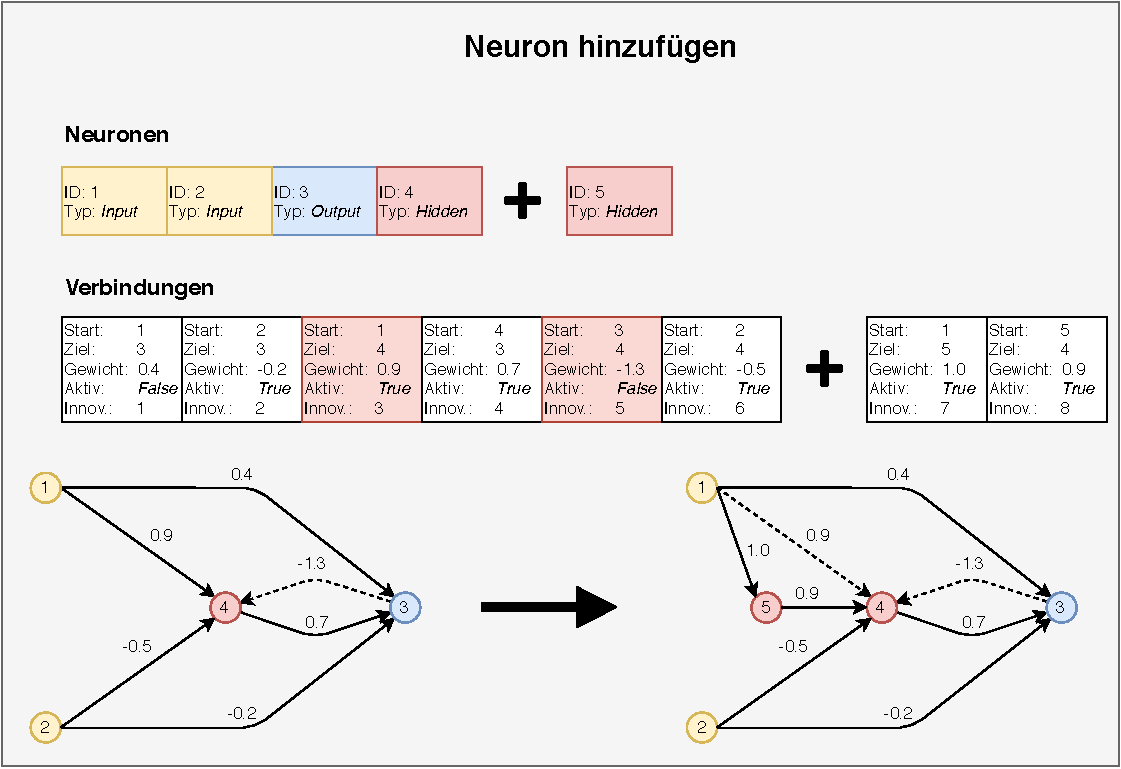
\includegraphics[width=1\textwidth]{./img/neat-AddNodeMutation.pdf} 
	\caption{Schematische Darstellung von einem Genom mit dazugehörigem Phänotyp}
	\label{fig:neat_add_node_mutation}
\end{figure}
\subsection{Reproduktion}
\label{subsec:neat_reproduction}
Das Ergebnis der in Kapitel \ref{subsec:neat_mutation} vorgestellten Mutationen ist eine Population mit verschieden Genomen, welche unterschiedliche Gewichte und Strukturen haben können. Dies ist die schwierigste Form des in Kapitel \ref{subsec:competing_convention_problem} vorgestellten \emph{competing convention} Problems und macht das Erstellen von Nachkommen besonders schwierig.\\
\ac{NEAT} löst dieses Problem, indem es den historischen Ursprung von jeder strukturellen Mutation überwacht. Haben zwei Verbindungen denselben Ursprung, haben sie in der Vergangenheit dieselbe Struktur repräsentiert, auch wenn sie inzwischen unterschiedliche Gewichte haben. Zu diesem Zweck besitzt jede Verbindungen die im Kapitel \ref{subsec:neat_encoding} erwähnte Innovationsnummer. Jedes Mal, wenn eine neue Verbindung entsteht, wird ein globaler Zähler inkrementiert und der Wert als Innovationsnummer der Verbindung verwendet. Abbildung (TODO ABBOLDUNG) zeigt die Zuweisung beispielhaft. Die erste Mutation, welche nur eine neue Verbindung herstellt, hat die Innovatiosnummer X zugewiesen bekommen. Wenn im Folgenden ein neues Neuron mit zwei weiteren Verbindungen hinzugefügt wird, erhalten diese die Nummern Y und Z. Werden Verbindungen von einem Genom in der Reproduktiosnphase für die Nachkommen ausgewählt, wird auch die Innovationsnummer übertragen. Somit ist auch bei den nachfolgenden Generationen ersichtlich, was der historische Ursprung einer Verbindung ist. Tritt durch Zufall dieselbe Mutation in einer Generation mehrfach auf, erhalten die neuen Verbindungen dieselben Innovationsnummern. Hierfür müssen alle aufgetretenen Mutation einer Generation zwischengespeichert werden. \\
Die Innovationsnummern können nicht nur ressourcensparend implementiert werden, sie machen auch das Erzeugen von Nachkommen in der Reproduktionsphase bedeutend einfacher, da beim Kreuzen von zwei Elternteilen keine aufwendige Strukturanalyse erforderlich ist. Abbildung (TODO ABBILDUNG) zeigt beispielhaft, wie ein Nachkommen aus zwei Elterngenomen $X$ und $Y$ entsteht. Die sogenannten \emph{maching genes} sind Verbindungen, deren Innovationsnummern in beiden Elterngenomen vorkommen. Beim Erstellen der Nachkommen wird für jede Verbindung in den \emph{matching genes} zufällig entschieden, aus welchem Elternteil diese übernommen wird. Die sogenannten \emph{disjoint genes} und \emph{excess genes} sind Verbindungen, die nur in einem Elternteil vorkommen. Zu den \emph{disjoint genes} gehören die Verbindungen, deren Innovationsnummer kleiner als die größte Innovationsnummer des zweiten Elterngenoms ist. Die \emph{excess genes} sind Verbindungen, deren Innovationsnummer größer als die höchste Innovationsnummer im anderen Elternteil ist. Beim Erzeugen von Nachkommen werden nur die \emph{excess genes} und \emph{disjoint genes} von dem Elternteil übernommen, welches den höheren Fitnesswert erzielt hat. Haben beide Elternteile den selben Wert, werden die Verbindungen von beiden übernommen.
Bei dieser Implementierung wird angenommen, dass der Schwellwert der Neuronen, wie in Kapitel (TODO KAPITE) erläutert, durch eine Verbindung zu einem \emph{Bias}-Neuron ausgedrückt wird. Dadurch enthalten die Neuronen keine spezifischen Informationen, die sich zwischen den Elterngenomen unterscheiden. Die Nachkommen übernehmen deshalb immer die Neuronen des Elternteils mit dem größeren Fitnesswert.
\subsection{Spezies}
\label{subsec:neat_species}
Die vorgestellten Arten der Mutation und die erfolgreiche Reproduktion ermöglichen es \ac{NEAT}, eine Population mit vielen verschiedenen Strukturen zu entwickeln. Dennoch reichen diese Faktoren nicht aus, da in der Praxis neue strukturelle Innovationen nur eine geringe Chance haben, langfristig integriert zu werden und es wahrscheinlicher ist, dass sie nach wenigen Generation aussterben. Die Gründe hierfür sind, dass kleinere \ac{KNN} schneller optimiert werden können als große und dass das Hinzufügen von neuen Neuronen und Verbindungen den Fitnesswert meistens initial senkt, auch wenn die neuen Strukturen für das erfolgreiche Lösen des Optimierungsproblems notwendig sind. Die Folge ist, dass die kleinen Genome anfänglich bessere Fitnesswerte erzielen, die größeren Genome nicht für die Reproduktion ausgewählt werden wodurch die strukturellen Innovationen wieder verloren gehen.
\\\\
Das Problem wird von \ac{NEAT} durch das Einführen von verschiedenen Spezies gelöst. Das Ziel ist, Genome, die sich strukturell ähnlich sind in einer Spezies zu gruppieren. Bei der Auswahl der Elterngenome für die Nachkommen muss ein Genom nicht mehr mit der ganzen Population konkurrieren, sondern nur noch mit den anderen Genomen der eigenen Spezies. Somit sind neue Innovationen erst einmal in ihrer Spezies vor dem Aussterben geschützt und können mit der Zeit optimiert werden. Für die Implementierung eines solchen Verfahrens wird eine Funktion benötigt, die messen kann, wie ähnlich oder unterschiedlich zwei Genome sind. Auch hier kann wie bei der Rekombination auf eine aufwendige Strukturanalyse verzichtet werden, da dies mit den bereits bekannten Innovationsnummern umsetzbar ist. Je mehr \emph{excess genes} und \emph{disjoint genes} zwei Genome besitzen, desto weniger evolutionäre Geschichte teilen sie und sind somit unterschiedlicher. Auch der Gewichtsunterschied ist ein wichtiger Faktor, wie in Kapitel \ref{subsec:competing_convention_problem} dargestellt. Die von \ac{NEAT} verwendete Formel, um die Kompatibilität $\delta$ zwischen zwei Genomen zu berechnen, ist im Folgenden abgebildet:
$$\delta=\frac{c_1E}{N}+\frac{c_2D}{N}+c_3 \cdot \overline{W}$$
Die Variablen $E$ und $D$ ergeben sich aus der Anzahl an \emph{excess genes} und \emph{disjoint genes}. $\overline{W}$ ist die durchschnittliche Gewichtsdifferenz der \emph{matching genes}. Die Faktoren $c_1$, $c_2$ und $c_3$ ermöglichen es die Wichtigkeit der einzelnen Komponenten je nach Optimierungsproblem zu justieren. $N$ steht für die Anzahl der Verbindungen im größeren Genom und normalisiert die Anzahl der \emph{excess genes} und \emph{disjoint genes}. Somit ist der Effekt auf den Kompatibilitätswert $\delta$ bei einer neuen Verbindung in großen Genomen gering und in kleinen sehr groß. Je nach Konfiguration kann für kleine Genome $N=1$ gelten.
\\\\
Die Zuordnung von neu erstellten Genomen zu einer Spezies erfolgt nach der Reproduktions- und Mutationsphase. Hierfür wird eine geordnete Liste mit allen verfügbaren Spezies benötigt. Jede Spezies wird durch ein Genom repräsentiert, welches in der vorherigen Generation ein Mitglied von dieser war. Bei der Zuordnung von einem Genom wird über die Liste der Spezies iteriert und zu jedem Repräsentanten der Kompatibilitätswert $\delta$ gebildet. Ist $\delta \leq \delta_t$, wobei $\delta_t$ ein konfigurierbarer Schwellwert ist, wird das Genom der Spezies zugeordnet und die Suche abgebrochen. Ist das Genom zu keiner Spezies kompatibel, wird eine neue erstellt und das Genom als Repräsentant gesetzt.
\\\\
Zum Erhalten von verschiedenen Strukturen muss verhindert werden, dass eine Spezies zu groß wird und die restlichen verdrängt, auch wenn viele der Mitglieder gute Fitnesswerte erzielen. Zusätzlich müssen insbesondere neue Spezies geschützt werden. Diese haben initial wenige Mitglieder und somit eine geringere Chance, als Elterngenome ausgewählt zu werden. Zum Lösen dieses Problems verwendet \ac{NEAT} sogenanntes \emph{explicit fitness sharing}, welches 1987 von \citeauthor{goldberg1987genetic} in ihrer Arbeit \cite{goldberg1987genetic} vorgestellt wurde. Jede Spezies bekommt bei der Reproduktion eine Anzahl an Nachkommen zugewiesen, welche proportional zur Fitness $f_{s}$ der Spezies ist. Diese ergibt sich aus der Summe aller angepassten Fitnesswerte $f'$ der Mitglieder. Der angepasste Fitnesswert $f'$ eines Genoms wird berechnet, indem die erreichte Fitness $f$ durch die Anzahl der Mitgliedern der Spezies geteilt wird. Ziel dieser Maßnahme ist, dass große Spezies im Vergleich zu kleinen benachteiligt werden. Hierdurch werden kleineren erfolgreichen Spezies entsprechend viele Nachkommen zugeordnet.
Ein Beispiel hierfür ist in Abbildung xy (TODO ABBILDUNG) dargestellt. Obwohl die zweite Spezies bedeutend weniger, jedoch gute Genome besitzt, werden ihr mehr Nachkommen zugewiesen. Würde die Anzahl der Nachkommen einer Spezies proportional zu der Summe der erreichten Fitnesswerte vergeben, hätte die kleinere Spezies weniger Nachkommen zugewiesen bekommen. 
\\\\
Ist der Fitnesswert $f_s$ von jeder Spezies berechnet und die Nachkommen proportional zugeteilt, beginnt die Reproduktion. Die Elterngenome werden hierfür zufällig aus der Mitgliederliste ausgewählt mit der Einschränkung, dass nur die besten $50\%$ der Genome ausgewählt werden. Sind alle Nachkommen erstellt, wird die ganze Population gelöscht und durch die Nachkommen ersetzt. Diese werden mit dem bereits vorgestellten Verfahren wieder den Spezies zugeordnet.
% TODO REF
% TODO EVENTUELL Oreilly vorher schon zitiert!!! Checken und text umbauen
\subsection{Starten mit einer minimalen Struktur}
\label{subsec:neat_minimal_structure}
Das Ziel von \ac{NEAT} sowie vieler anderer Optimierungsalgorithmen ist, eine Lösung in kürzester Zeit zu finden. Ein wichtiger Faktor ist hierbei die Größe des \ac{KNN}. Ein zu großes \ac{KNN} hat viele modifizierbare Verbindungsgewichte und Schwellwerte, welche nicht zur erfolgreichen Lösung benötigt werden. Trotzdem wird die Laufzeit des Algorithmus erhöht, da auch diese optimiert werden müssen. Ein zu kleines \ac{KNN} kann, wie in Kapitel (TODO REF XOR) veranschaulicht, unter Umständen nicht in der Lage sein, eine Lösung zu finden. Somit ist die richtige Größe des \ac{KNN} entscheidend für die schnelle Optimierung. Für Algorithmen, welche nur die Gewichte eines \ac{KNN} optimieren, muss diese Struktur von einem Menschen festgelegt werden. Meistens basiert dies auf Expertenwissen oder Erfahrung \cite{stanley2017oreilly}. Im Gegensatz hierzu stehen die \ac{TWEANN} Algorithmen, welche selbstständig eine gute Struktur bilden sollen. Diese starten oft mit einer initialen Population mit vielen verschiedenen zufällig erstellten Topologien mit dem Ziel, genetische Diversität zu bieten. Wie in Kapitel \ref{subsec:tweann} erläutert, ist dies oft ineffizient, da viele Strukturen nicht gebraucht werden und Zeit benötigt wird, diese zu entfernen.
\\\\
\ac{NEAT} hingegen startet mit einer Population, bei der alle Genome dieselbe minimale Struktur besitzen. Die entstehenden \ac{KNN} haben nur \emph{Input}- und \emph{Output}-Neuronen und keine \emph{Hidden}-Neuronen. Jedes \emph{Input}-Neuron besitzt eine Verbindungen zu jedem \emph{Output}-Neuron mit einem zufällig gewählten Gewicht. Neue Strukturen werden durch die vorgestellten Arten der Mutation hinzugefügt, von denen nur diejenigen langfristig integriert werden, welche den Fitnesswert erhöhen. Somit ist die Existenz von jeder Struktur in einem Genom gerechtfertigt. Insgesamt gibt dies \ac{NEAT} einen Vorteil bezüglich der Evaluationszeit gegenüber anderen \ac{TWEANN} Algorithmen, da die Anzahl der zu optimierenden Parameter und somit die Dimensionen des Suchraums minimiert sind.
% !TeX spellcheck = de_DE
\section{Parallelisierung}
\label{sec:parallel}
In den vorherigen Kapiteln ist der Ablauf und die Funktionsweise von neuroevolutionären Algorithmen erläutert. Die benötigte Ausführungszeit ist von der Größe des \ac{KNN}, der Komplexität des Problems und der Populationsgröße abhängig. Für die Optimierung großer \ac{KNN} können trotz Verwendung aktueller Hardware Trainingszeiten von mehreren Stunden oder Tagen benötigt werden \cite{such2017deep}. Diese Zeit kann durch Weiterentwicklungen von einzelnen Prozessoren zunehmend verringert werden. Allerdings ist der Leistungsanstieg von neuen Prozessorgenerationen nicht ausreichend, um die benötigte Rechenzeit von solch anspruchsvollen Anwendungen massiv zu senken und skaliert somit in diesem Anwendungskontext schlecht. Zusätzlich ist die Aktualität der Prozessoren mit großem finanziellen Aufwand verbunden \cite{swann2002maximum}. Die Parallelisierung ist ein weiterer Ansatz, um die benötigte Ausführungszeit zu verringern. Hierbei wird ein großes Problem in mehrere kleine, voneinander unabhängige Teilprobleme zerlegt. Diese können dann auf verschiedenen Prozessoren gleichzeitig berechnet werden \cite{swann2002maximum}. Häufig wird in diesem Zusammenhang auch der Begriff \ac{HPC} verwendet, auf welchen im Folgenden näher eingegangen wird.

\subsection{High Performance Computing}
Das \ac{HPC} beschäftigt sich mit verschiedenen Bereichen der parallelen Programmierung. Hierzu gehören unter anderem die benötigte Software, Programmiersprachen, Tools sowie die Hardware. Zusammenfassend ist festzustellen, dass sich der Bereich \ac{HPC} mit der Forschung, Entwicklung und dem Betreiben von \acp{SC} beschäftigt. Dies sind Cluster, welche aus mehreren Millionen \acp{CPU} bestehen und zum Lösen von verschiedenen parallelisierbaren Problemen aus Forschung und Industrie verwendet werden können \cite{nielsen2016introduction}. Eine Liste mit den $500$ leistungsfähigsten \acp{SC} ist in Quelle \cite{top500} zu finden. Stand Juni 2020 ist der leistungsfähigste \ac{SC} in Japan, welcher über sieben Millionen Prozessoren besitzt und eine Leistung von über $500.000$ TFlops bietet. Aufgrund hoher Kosten, die unter anderem durch den Stromverbrauch entstehen, sind \ac{SC} für viele Probleme nicht rentabel. Dennoch gibt es einige Anwendungsszenarien für solche Systeme.
\\\\
Häufig werden \ac{SC} für verschiedene Simulationen eingesetzt, deren Durchführung in realer Umgebung zu teuer oder zu gefährlich ist und für die als Beispiel ein Flugzeugabsturz oder die Auswirkungen nuklearer Waffen zu benennen sind. Ein weiterer Grund für den Einsatz von SC liegt vor, wenn die Berechnung oder Simulation auf einem gewöhnlichen Gerät zu viel Zeit benötigt oder wenn das Ergebnis nur eine gewisse Zeit gültig bzw. verwendbar ist. Ein Problem dieser Kategorie ist beispielsweise die Wettervorhersage. Ist es nicht möglich, das Ergebnis rechtzeitig zu erhalten, ist die Vorhersage obsolet. Nicht zuletzt ist auch die Analyse von großen Datenmengen, die nicht auf einem einzelnen Gerät effizient durchführbar ist, eine Einsatzmöglichkeit von \ac{SC} \cite{nielsen2016introduction}.

\subsubsection{Architektur}
\label{subsubsec:hpc_architecture}
Die Architekturen von \ac{HPC} Systemen sind einer von zwei Kategorien zuzuordnen, welche als \emph{shared memory} und \emph{distributed memory} bezeichnet werden. Bei der \emph{shared memory} Architektur verwenden typischerweise alle Prozessoren des Systems denselben Programmspeicher, der auch als \ac{RAM} bezeichnet wird. Die Kommunikation zwischen den Prozessoren ist in vielen Fällen durch \ac{OpenMP} realisiert \cite{nielsen2016introduction}. Diese Art der Parallelisierung kann auch auf Computersystemen angewendet werden, die für den Massenmarkt produziert wurden. Moderne \acp{CPU} besitzen auf demselben Chip mehrere physische Prozessoren, welche zur Parallelisierung von verschiedenen Anwendungen verwendet werden können und häufig die Ausführungszeit bedeutend reduzieren. 
\\\\
Die Alternative hierzu ist die \emph{distributed memory} Architektur, bei der jeder Prozessor seinen eigenen \ac{RAM} besitzt. Im Gegensatz zu \emph{shared memory} Architekturen können die Prozessoren dieser Art nicht auf Speicherbereiche von anderen Prozessoren zugreifen. Um eine Kommunikation zwischen den einzelnen Prozessoren zu ermöglichen, müssen sie explizite Nachrichten untereinander austauschen. Die Ausführungsgeschwindigkeit bzw. die Effizienz der parallelisierten Anwendung ist nicht nur von den einzelnen Prozessoren abhängig, sondern auch von der Latenz, Bandbreite und Netztopologie. Die Latenz beschreibt hierbei die Zeit, welche benötigt wird, eine Kommunikation zu initiieren, die Bandbreite die Übertragungsgeschwindigkeit der Daten. Neben diesen beiden Architekturen gibt es noch weitere Formen, welche auch \acp{GPU} nutzen können \cite{nielsen2016introduction}. Auf diese wird nicht weiter eingegangen, da in dieser Arbeit ein System mit einer \emph{distributed memory} Architektur verwendet wird.

\subsubsection{Beowulf-Cluster}
\label{subsubsec:beowulf_cluster}
Durch enorme Kosten, die in der Anschaffung spezialisierter Hardware \cite{brown2004engineering} sowie im Betrieb eines \ac{SC} \cite{nielsen2016introduction} entstehen, ist ein solches System für die meisten Unternehmen, Universitäten oder Hochschulen finanziell nicht tragbar. Dennoch kann der Einsatz kleinerer Cluster zum Beispiel in der Lehre oder für weniger rechenaufwendige Probleme, welche trotzdem von einer Parallelisierung profitieren, sinnvoll sein. 
\\\\
In einem solchen Szenario sind sogenannte Beowulf-Cluster eine mögliche Lösung. Diese haben zwar bedeutend weniger Leistung, sind dafür aber in der Anschaffung sowie im Betrieb um ein Vielfaches günstiger und eignen sich somit auch für Privatpersonen \cite{adams2008microwulf}. Diese Cluster zeichnen sich in Abgrenzung zu professionellen \ac{SC} unter anderem dadurch aus, dass die Hardware für den eigentlichen Beowulf-Cluster aus serienmäßig für den Massenmarkt produzieren Geräten zusammengesetzt werden kann. Gleiches gilt auch insofern für die Netzwerkinfrastruktur, dass ein Cluster aus mehreren Desktopgeräten bestehen kann, welche über ein Ethernet-Netzwerk miteinander verbunden sind. Weitere Anforderungen sind, dass alle Geräte des Clusters nur \emph{Open-Source}-Software verwenden, das Netzwerk exklusiv für die Kommunikation des Beowulf-Clusters reserviert ist und das Aufgabengebiet im Bereich des \ac{HPC} liegt \cite{brown2004engineering}. Diese Anforderungen müssen für einen klassischen Beowulf-Cluster erfüllt sein, dennoch gibt es verschiedene abgewandelte Varianten für andere Einsatzszenarien.
\\\\
Typischerweise basiert das Betriebssystem der einzelnen als \emph{Nodes} bezeichneten Geräte auf Linux, worin sich eine Eigenschaft verdeutlicht, welche auf die meisten Beowulf-Cluster zutrifft, aber keine Voraussetzung ist. Häufig wird ein \emph{Node} als \emph{Master} ausgewählt, der als Schnittstelle zwischen dem eigentlichen Cluster und der externen Umgebung dient, die restlichen \emph{Nodes} werden als \emph{Slaves} bezeichnet. So kommt es häufig vor, dass der \emph{Master} über eine angeschlossene Tastatur und einen Bildschirm verfügt, welche eine Interaktion mit dem Cluster ermöglichen. Zusätzlich hat dieser häufig als einziges Gerät neben der Verbindung zu den \emph{Slaves} auch eine externe Netzwerkanbindung. Dies wird benötigt, da der \emph{Master} in der Regel viele organisatorische Aufgaben übernimmt. Beispiel hierfür kann das Bereitstellen und die Synchronisation von Dateien im Netzwerk sein \cite{brown2004engineering}.
\\\\
Aufgrund der vergleichsweise niedrigen Kosten sowie der einfachen Anschaffung und Inbetriebnahme bieten sich solche Cluster für viele verschiedene Projekte an. Auch in dieser Arbeit wird ein Beowulf-Cluster verwendet, auf dessen Installation und Konfiguration in Kapitel \ref{sec:test_env_parallel} eingegangen wird.

\subsubsection{MPI und MapReduce}
\label{subsubsec:mpi_and_mapreduce}
Für eine erfolgreiche Parallelisierung in einem \emph{distributed memory} System, wie zum Beispiel in einem Beowulf-Cluster, müssen sich die einzelnen Prozessoren untereinander synchronisieren sowie Nachrichten austauschen können. Hierfür gibt es verschiedene Bibliotheken, welche einen Großteil dieser Funktionen bereitstellen. Beispiele hierfür sind \ac{MPI} und \emph{MapReduce}. Diese unterscheiden sich in ihrer Funktionalität und der Umgebung, in welcher sie eingesetzt werden \cite{nielsen2016introduction}.
\\\\
Die Verwendung von \ac{MPI} in dieser Arbeit, welches in Kapitel \ref{subsec:mpi} genauer erläutert wird, ist unter anderem in seinem Vorteil begründet, dass eine Vielzahl verschiedener Kommunikations- und Synchronisationsoperatoren implementiert sind, welche flexibel an viele Anforderungen angepasst werden können. Allerdings besteht keine Fehlertoleranz gegenüber Hardware- und Netzwerkfehlern. Treten diese auf, bricht die Ausführung der gesamten Anwendung ab und nicht gespeicherte Zwischenergebnisse gehen verloren. Bezüglich diesen Aspekts bietet die Alternative \emph{MapReduce} einen Vorteil, da diese Fehler automatisch verarbeiten kann. Nachteil gegenüber \ac{MPI} ist, dass nicht so viele verschiedene, flexible Funktionen der Parallelisierung geboten werden \cite{nielsen2016introduction}.

\subsection{MPI}
\label{subsec:mpi}
Wie in den vorherigen Kapiteln erläutert, müssen in einem parallelen System die Prozessoren miteinander kommunizieren können. Vor allem bei Systemen mit einer \emph{distributed memory} Architektur wird häufig \ac{MPI} verwendet, welches ein anerkannter Standard im Bereich \ac{HPC} ist. Zusätzlich kann \ac{MPI} auch auf \emph{shared memory} Architekturen angewendet werden. Die erste Version des Standards wurde bereits 1991 entwickelt \cite{nielsen2016introduction}. Im Jahr 2008 wurde die derzeit aktuelle Version 3 veröffentlicht. Bevor die verschiedenen Funktionen von \ac{MPI} vorgestellt werden, wird zunächst auf einige Besonderheiten eingegangen. Der Standard \ac{MPI} ist keine konkrete Implementierung, sondern ein \ac{API}, welches nur die grundsätzliche Funktionsweise sowie einige Basisoperationen definiert \cite{nielsen2016introduction}. Einer der sich ergebenden Vorteile ist darin zu verdeutlichen, dass die Implementierung des Standards nicht an eine einzelne Programmiersprache geknüpft ist \cite{nielsen2016introduction}. Dies gibt Herstellern die Möglichkeit, ihre eigene Implementierung in jeder gewünschten Sprache umzusetzen. Hieraus sind viele kommerzielle Produkte entstanden, aber mit \emph{MPICH} und \emph{Open MPI} auch zwei bekannte \emph{open source} Lösungen. Diese können als Bibliotheken in andere Projekte eingebunden werden und vereinfachen die Entwicklung einer parallelen Anwendung enorm, da verschiedene \emph{low-level} Funktionen, wie beispielsweise die Netzwerkkommunikation, bereits implementiert sind. Des Weiteren ermöglicht der \ac{MPI} Standard eine hohe Portabilität, da Implementierungen mit wenig Aufwand ausgetauscht werden können und auf einer Vielzahl von Systemen lauffähig sind \cite{dalcin2008mpi}.
\\\\
Die Funktionen von \ac{MPI} können heutzutage in verschiedenen Sprachen, wie zum Beispiel Java, C, C++, Python und Fortran verwendet werden \cite{nielsen2016introduction}. Im Folgenden wird auf die wichtigsten Grundfunktionen von \ac{MPI} eingegangen. Der Beispielcode ist in der Sprache Python und der Bibliothek \emph{mpi4py} aus Quelle \cite{dalcin2008mpi} implementiert. Diese werden auch im weiteren Verlauf dieser Arbeit verwendet.
% TODO Check if code examples are really used
\subsubsection{Prozessorgruppen}
Bevor die verschiedenen Kommunikations- und Synchronisationsmöglichkeiten vorgestellt werden, muss der grundlegende Ablauf eines auf \ac{MPI} basierenden Programms betrachtet werden. Beim Starten eines solchen Programms wird auf jedem der beteiligten Prozesse, welche in einer Konfigurationsdatei spezifiziert sind, eine Kopie des Programms ausgeführt. Eine grundlegende Voraussetzung ist, dass das Programm auf allen beteiligten \emph{Nodes} vorliegt. 
\\\\
Die sogenannten \emph{Communicators}, im Programmcode auch häufig mit \emph{COMM} abgekürzt, sind Gruppen von verschiedenen Prozessen, welche miteinander kommunizieren können. Beim initialen Starten des Programms wird nur eine Prozessgruppe erstellt, welche alle beteiligten Prozesse enthält und als \emph{MPI\_COMM\_WORD} bezeichnet wird. Jeder Prozess in einem \emph{Communicator} wird  durch einen Rang zwischen $0$ und $P-1$ identifiziert, wobei $P$ die Anzahl an Prozessen ist \cite{nielsen2016introduction}. Der Rang sowie die Anzahl der Prozesse können im Programmcode angefragt und als Grundlage für verschiedene Entscheidungen genutzt werden. Ein Beispiel hierfür ist in Abbildung \ref{fig:example_process_group} dargestellt. Der gegebene Programmabschnitt wurde mit zwei Prozessoren ausgeführt. An der Ausgabe ist erkennbar, dass die Anweisung \emph{print()} von jedem Prozess einmal aufgerufen wird und sich lediglich die Variable \emph{rank} unterscheidet. 
\begin{figure}
	
	\begin{python}
		from mpi4py import MPI
		
		comm = MPI.COMM_WORLD
		rank = comm.Get_rank()
		size = comm.Get_size()
		
		print("Hello world, Rank:", rank, ", Size:", size)
		
		>>> Hello world, Rank: 1, Size: 2
		>>> Hello world, Rank: 0, Size: 2
	\end{python}
	\caption{\emph{HelloWord} MPI Programm in Python}
	\label{fig:example_process_group}
\end{figure}



% MPI Communicaor, splittet Processe in Auf, 
% Aktuell Version 3
% Ursprünglich 80 Personen und 30 Organisationen, Attraktiv because Protability and Scalability, Distributed and Shared Memory Multiprocesses
% Standard defacto von HPC
% Blocking Non Blocking
\subsubsection{Point-to-Point Kommunikation}
\label{subsubsec:point_to_point_communication}
Typischerweise wird \ac{MPI} unter anderem zum Austauschen von Nachrichten verwendet. Bei der in diesem Abschnitt vorgestellten, sogenannten \emph{Point-to-Point} Kommunikation sendet ein Prozess entweder synchron oder asynchron Daten an einen anderen \cite{nielsen2016introduction}. Abbildung \ref{fig:example_point_to_point} zeigt ein Beispiel für die synchrone Kommunikation, in der die \emph{send()} und \emph{recv()} Funktion zum Einsatz kommen. Die \emph{send()} Funktion versendet Daten an einen anderen Prozess. Als Parameter müssen die zu sendenden Daten und das Ziel übergeben werden. Dieses wird durch den entsprechenden Rang identifiziert. Optional kann der Funktion noch ein \emph{tag} übergeben werden, welches zusätzliche Informationen zu den Daten enthält. Beispielsweise kann dieses verwendet werden, um dem Zielprozess zu signalisieren, wie die Daten verarbeitet werden sollen. Die \emph{recv()} Funktion wird zum Empfangen der Daten verwendet. Diese kann prinzipiell ohne Parameter aufgerufen werden, sodass jede Nachricht von jedem Prozess akzeptiert wird. Sollen spezielle Nachrichten mit einem gewissen \emph{tag} oder von einem spezifischen Prozess empfangen werden, ist dies durch Übergeben von weiteren Parametern möglich. Dies kann wichtig sein, wenn Nachrichten beispielsweise in einer gewissen Reihenfolge empfangen werden müssen. 
\begin{figure}
	\begin{python}
		from mpi4py import MPI
		
		comm = MPI.COMM_WORLD
		rank = comm.Get_rank()
		size = comm.Get_size()
		
		if rank == 0:
			data_to_send = 42
			comm.send(data_to_send, dest=1)
			print("Data sent: ", str(data_to_send))
		elif rank == 1:
			data_recv = comm.recv()
			print("Data received: " + str(data_recv))
			
		>>> Data sent:  42
		>>> Data received: 42
	\end{python}
	\caption{\emph{Point-to-Point} Kommunikation mit \ac{MPI} in Python}
	\label{fig:example_point_to_point}
\end{figure}
\\ \noindent
Eines der Probleme, das potenziell durch die synchrone Kommunikation verursacht wird, betrifft die Effizienz, da sowohl die \emph{send()} als auch \emph{recv()} Funktion die weitere Ausführung des Programmcodes blockieren, bis die Übertragung erfolgreich abgeschlossen ist. Sollte einer der beiden Prozesse ausgelastet sein, wird der andere auf ihn warten und in dieser Zeit keine Berechnungen durchführen \cite{nielsen2016introduction}. Kommen diese Wartezeiten häufig und lange vor, kann dies die Performanz des Systems stark beeinträchtigen. Ein weiteres Problem besteht darin, dass Fehler im Programmcode zu \emph{Deadlocks} führen können. Eine solche Situation kann entstehen, wenn zwei Prozesse eine Nachricht vom jeweils anderen erwarten und daher nicht mit der Programmausführung fortfahren \cite{nielsen2016introduction}. Da kein Prozess eine Nachricht schicken wird, muss das Programm in einem solchen Fall extern manuell beendet werden und alle nicht gespeicherten Zwischenergebnisse gehen verloren. Um diese Probleme zu umgehen, kann die asynchrone Variante der \emph{Point-to-Point} Kommunikation verwendet werden, welche mit den Funktionen \emph{isend()} und \emph{irecv()} implementiert ist. Möchte ein Prozess Daten senden bzw. empfangen und ist der Kommunikationspartner noch nicht bereit, wird mit der Ausführung des Programmcodes fortgefahren. Wenn der Kommunikationspartner letztendlich für die Übertragung bereit ist, wird diese automatisch gestartet \cite{nielsen2016introduction}. 

\subsubsection{Gruppenkommunikation}
Der \ac{MPI} Standard definiert nicht nur die \emph{Point-to-Point} Kommunikation, sondern auch verschiedene Formen der Gruppenkommunikation. Diese können in einigen Fällen bedeutend effizienter sein, als Nachrichten mit allen Prozessen einzeln auszutauschen. Einige der wichtigsten Operationen sind die \emph{Broadcast}, \emph{Scatter}, \emph{Gather} und \emph{Reduce} Funktion, welche beispielhaft in Abbildung \ref{fig:mpi_group_communication} dargestellt sind \cite{dongarra1995introduction}.
\begin{figure}[!h]
	\centering
	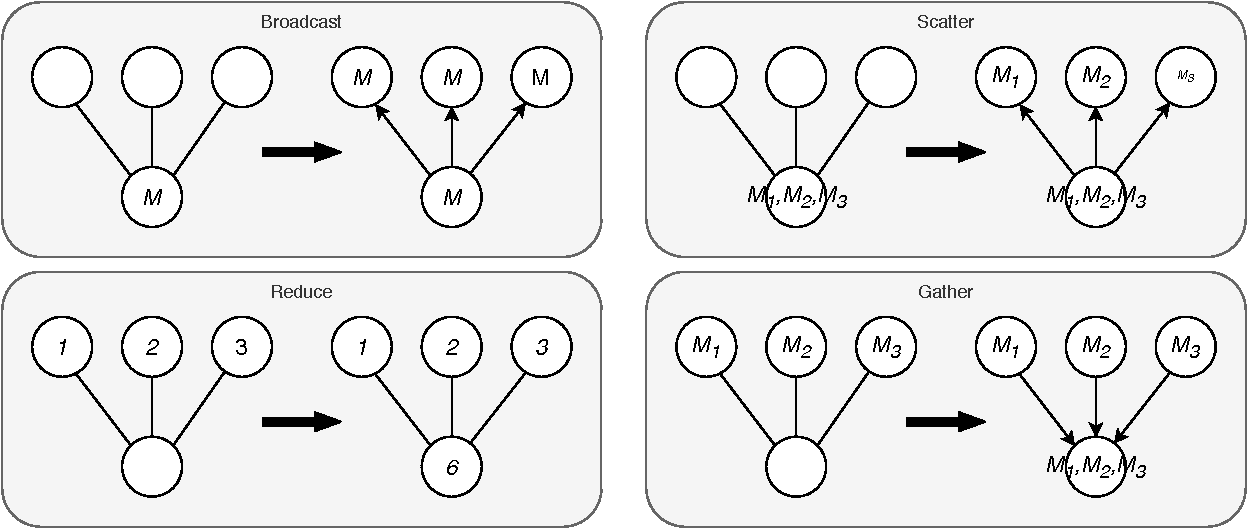
\includegraphics[width=1\textwidth]{./img/mpi_group_communication.pdf} 
	\caption{Schematische Darstellung der \emph{Broadcast}, \emph{Scatter}, \emph{Gather} und \emph{Reduce} Funktion in MPI}
	\label{fig:mpi_group_communication}
	% TODO Eventuell Pfeile bei reduce hinzufügen?
\end{figure}
\\ \noindent
Mit der \emph{Broadcast} Funktion kann ein Prozess eine Nachricht $M$ an alle anderen beteiligten Prozesse senden \cite{dongarra1995introduction}. Diese einfache Operation wird in vielen Fällen benötigt, wenn beispielsweise der \emph{Master} Prozess in einem Cluster Daten an alle \emph{Slaves} senden muss. Mit der \emph{Scatter} Funktion kann ein Prozess die Elemente einer Liste bzw. eines Arrays gleichmäßig an die anderen Prozesse verteilen, sodass jeder Empfänger nur einen Teil der Daten erhält \cite{nielsen2016introduction}. Diese Operation kann eingesetzt werden, wenn für jedes Element der Liste eine vom Rest unabhängige Berechnung durchgeführt werden muss. Zwar wäre es in einem solchen Szenario auch möglich, die \emph{Broadcast} Funktion zu verwenden und dann basierend auf dem Rang die Berechnung durchzuführen, aber bei der \emph{Scatter} Funktion werden insgesamt weniger Daten übertragen und somit eine geringere Bandbreite benötigt. Das Pendant zur \emph{Scatter} Funktion ist die \emph{Gather} Funktion. Hierbei erhält ein Prozess von allen anderen eine Nachricht $M_i$ und aggregiert diese in einer Liste oder einem Array \cite{nielsen2016introduction}. Die \emph{Scatter} und \emph{Gather} Funktionen werden häufig zusammen verwendet. Mit der \emph{Scatter} Funktion können die Daten an die verschiedenen Prozesse verteilt werden, diese berechnen ihre Ergebnisse, welche zuletzt mit der \emph{Gather} Funktion wieder gesammelt werden. Die letzte hier vorgestellte Funktion wird \emph{Reduce} genannt. Mit dieser können verschiedene globale Berechnungen mit einem binären kommutativen Operator durchgeführt werden \cite{nielsen2016introduction}. Eine Rechenoperation ist kommutativ, wenn für alle $a$ und $b$ einer Menge $M$  die Gleichung $a*b=b*a$ gilt \cite{walz2011brueckenkurs}. In Abbildung \ref{fig:mpi_group_communication} wird die Summe berechnet, aber \ac{MPI} bietet darüber hinaus andere Standardoperatoren, wie die Berechnung des Produkts, Minimums oder Maximums \cite{nielsen2016introduction}. 
\\\\
\ac{MPI} bietet noch weitere Arten der Gruppenkommunikation, auf welche an dieser Stelle nicht ausführlich eingegangen wird. Die \emph{AllGather} Funktion kombiniert die \emph{Gather} Funktion mit einem anschließenden \emph{Broadcast} des Ergebnisses. Bei der \emph{AllToAll} Funktion besitzt jeder Prozess eine Liste und sendet jeweils ein Element an jeden anderen Prozess \cite{dongarra1995introduction}. Eine spezielle Art der Gruppenkommunikation sind die sogenannten Synchronisationsbarrieren, an denen die Ausführung der einzelnen Prozesse angehalten wird, bis alle Teilnehmer diese erreicht haben \cite{nielsen2016introduction}. Abschließend sind zwei Anmerkungen zu nennen, welche für die verschiedenen Arten der Gruppenkommunikation wichtig sein können. Erstens ist jede dieser Operationen nur als synchrone Funktion verfügbar. Die zweite Anmerkung betrifft die Synchronisationsbarrieren. Bei vielen Implementierungen haben Funktionen wie der \emph{Broadcast} einen Synchronisationsseiteneffekt. Dies ist durch den \emph{MPI} Standard möglich, jedoch keine Voraussetzung und kann somit die Portierung von Projekten beeinflussen, die von diesen Seiteneffekten abhängig sind \cite{dongarra1995introduction}.

\subsection{Performance}
\label{subsec:basics_performance}
% Eventuell load balancing, wichtig
Das Erstellen eines gut parallelisierten Algorithmus ist häufig bedeutend schwieriger als das Erstellen desselben in einer sequenziellen Variante. Der Grund hierfür ist, dass zwar jeder parallele Algorithmus sequenziell ausführbar ist, indem die unabhängigen Teilaufgaben nacheinander abgearbeitet werden, dies aber umgekehrt nicht möglich ist. Um gute Ergebnisse zu erzielen, muss der parallelisierte Algorithmus häufig neu erstellt oder umstrukturiert werden. \cite{nielsen2016introduction}. Dieses Kapitel stellt Methoden vor, mit welchen die tatsächliche und maximal zu erwartende Performance eines parallelen Algorithmus berechnet werden kann. 
\\\\
Bevor auf die genauen Berechnungen eingegangen wird, sei angenommen, dass die serielle Ausführung eines Algorithmus $t_{seq}$ lange dauert und dass $t_q$ die Zeit angibt, welche derselbe parallele Algorithmus mit $P$ Prozessoren benötigt. Der sogenannte \emph{SpeedUp} gibt an, um welchen Faktor die parallele Ausführung eines Programms schneller ist. Berechnet wird dies mit $SpeedUp(P)=\frac{t_{seq}}{t_P}$ \cite{nielsen2016introduction}. Der \emph{SpeedUp} gibt nicht an, wie gut oder schlecht die tatsächliche Parallelisierung ist. Hierfür wird die Effizienz $e$ benötigt, welche mit $e=\frac{SpeedUp(P)}{P}$ berechnet wird. An dieser kann abgelesen werden, wie gut die parallele Ausführung tatsächlich ist. Der berechnete Wert liegt meistens zwischen $0$ und $1$, wobei ein niedriger Wert ein dafür Indiz ist, dass durch die Parallelisierung und eventuelle Kommunikation viel zusätzlicher Rechenaufwand entsteht. Dementsprechend zeigt ein hoher Wert, dass wenig zusätzlicher Aufwand entsteht und die Parallelisierung effizient erfolgt. In seltenen Fällen ist es sogar möglich, dass höhere Werte als $1$ erzielt werden, was einem \emph{super-linear SpeedUp} entspricht. Dies kann vorkommen, wenn beispielsweise mehrere Prozesse denselben \emph{Cache} verwenden. Hierbei ist es möglich, dass ein Prozess Rechenzeit einsparen kann, indem er ein Ergebnis aus dem \emph{Cache} wiederverwendet, das ein anderer Prozess berechnet hat \cite{nielsen2016introduction}.
\\\\
Mit den vorgestellten Formeln lassen sich der \emph{SpeedUp} und die Effizienz berechnen, sie geben allerdings keine Auskunft darüber, was der höchst mögliche \emph{SpeedUp} bzw. die kürzeste Ausführungszeit ist. Um diese zu berechnen, gibt es zwei Theoreme, welche unter den Begriffen \emph{Amdahl's Law} und \emph{Gustafson's Law} bekannt sind \cite{nielsen2016introduction}. 
\\\\
\emph{Amdahl's Law} wurde 1967 von Gene Amdahl in seiner Arbeit in Quelle \cite{amdahll1967validity} beschrieben. Die im Folgenden vorgestellten Formeln wurden erst später hieraus abgeleitet \cite{amdahll1967validity}. Angenommen wird ein Algorithmus bestehend aus zwei Teilen, bei dem der erste Teil $\alpha_{seq}$ rein sequenziell und der zweite Teil $\alpha_{par}$ parallelisierbar ist. Weiterhin wird angenommen, dass $\alpha_{seq}+\alpha_{par}=1$ ist und dass $t_1$ die Zeit angibt, welche ein einzelner Prozess zum Ausführen eines Programmabschnittes benötigt. Die Ausführungszeit $t_P$ eines solchen parallelisierten Programms mit $P$ Prozessen kann mit $t_P=\alpha_{seq} \cdot t_1 + \alpha_{par} \cdot \frac{t_1}{P}$ berechnet werden. Um den höchsten erreichbaren \emph{SpeedUp} zu berechnen wird angenommen, dass $t_1=t_{seq}$ gilt und der erhaltenen Wert $t_P$ in die bereits vorgestellte Formel für die Berechnung des \emph{SpeedUps} eingesetzt wird. Hierdurch ergibt sich die bekannte Formel von \emph{Amdahl's Law} \cite{nielsen2016introduction}: 
$$SpeedUp(P)=\frac{1}{\alpha_{seq}+\frac{\alpha_{par}}{P}}$$
Angenommen, es gäbe unendlich viele Prozessoren ($P \rightarrow \infty$), dann ist die Ausführungszeit des parallelisierbaren Programmteils vernachlässigbar gering, sodass nur der sequenzielle Anteil das Ergebnis maßgeblich beeinflusst und somit gilt \cite{nielsen2016introduction}:
$$\lim _{P \rightarrow \infty} SpeedUp(P)=\frac{1}{\alpha_{seq}}$$
Ist ein Algorithmus beispielsweise zu $95\%$ parallelisierbar und dementsprechend zu $5\%$ seriell, dann beträgt der maximale \emph{SpeedUp} für diesen $20$. \emph{Amdahl's Law} gilt unter der Annahme, dass bei steigender Prozessanzahl der Rechenaufwand der zu lösenden Aufgabe konstant bleibt, was auf viele Anwendungsszenarien zutrifft \cite{nielsen2016introduction}. Im Gegensatz hierzu steht das \emph{Gustafson's Law}, welches von John Gustafson stammt. Dieser argumentiert, dass \emph{Amdahl's Law} parallelen Systemen nicht gerecht würde, da der eigentliche Vorteil von diesen die Bearbeitung von größeren Datenmengen in derselben Zeit sei. In diesem Fall wird mit steigender Prozessanzahl ebenfalls der Rechenaufwand erhöht. Dies ermöglicht es, höhere \emph{SpeedUp} Werte zu erzielen \cite{hill2008amdahl}.




















